\chapter{phase transitions: criticality, universality, and scaling}
\begin{itemize}
	\item 热力学系统可以分为两类: noninteracting \& interacting.
	
	\item noninteracting 的系统包括: the specific heat of gases (section \ref{1.2} and \ref{6.4}); the specific heat of solids (section \ref{7.4}); chemical equilibrium in an ideal gas or a dilute solution (section \ref{6.5}); condensation of an ideal Bose gas (section \ref{7.1} and \ref{7.2}); spectral distribution of the blackbody radiation (section \ref{7.3}); the free electron theory of metals (section \ref{8.3}); the phenomenon of paramagnetism (section \ref{3.7} and \ref{8.2}).
	\begin{itemize}
		\item 除了 Bose--Einstein condensation 之外, 所有这些系统的 thermodynamic functions 都是光滑的.
	\end{itemize}
	
	\item interacting 的系统包括: the condensation of gases; the melting of solids; the coexistence of phases (especially near a critical point); mixtures and solutions (包括 the onset of phase separation); ferromagnetism and antiferromagnetism; the order--disorder transitions in alloys; the superfluid transition from liquid He I to liquid He II; transition from a normal to a superconducting material.
	\begin{itemize}
		\item interacting 的系统, 经常会遇到 thermodynamic functions 具有 analytic discontinuities or singularities 的情况, 相应地, 会遇到各种 phase transitions.
	\end{itemize}
\end{itemize}

\section{general remarks on the problem of condensation}
\begin{itemize}
	\item 对任何热力学系统, 都有
	\begin{equation}
		\Big( \frac{\partial P'}{\partial v} \Big)_{V, T} = - \frac{k_B T}{v^2} \frac{\braket{N}}{\braket{(\Delta N)^2}} \leq 0,
	\end{equation}
	其中 $P'$ 定义为
	\begin{equation}
		P' := \frac{k_B T}{V} \ln Z_\text{GC} \equiv - \frac{\Phi_\text{G}}{V},
	\end{equation}
	对于 homogeneous system (注意 multiphase systems 也可以是 homogeneous, 但要忽略表面效应) 有 $P' = P$.
	
	\begin{tcolorbox}[title=calculation:]
		注意到
		\begin{equation}
			- \frac{V}{N^2} \Big( \frac{\partial P'}{\partial v} \Big)_{T, V} = \Big( \frac{\partial P'}{\partial N} \Big)_{T, V} = - \frac{1}{V} \Big( \frac{\partial \Phi_\text{G}}{\partial N} \Big)_{T, V},
		\end{equation}
		且
		\begin{equation}
			\Big( \frac{\partial \Phi_\text{G}}{\partial N} \Big)_{T, V} = - N \Big( \frac{\partial \mu}{\partial N} \Big)_{T, V} = - \frac{N}{\big( \frac{\partial N}{\partial \mu} \big)_{T, V}} = - \frac{N}{\beta \braket{(\Delta N)^2}},
		\end{equation}
		最后一个等号用到了 \eqref{4.4.1}.
	\end{tcolorbox}
	
	\item 注意到, 在某些区间 $\braket{(\Delta N)^2} \sim O(N^2)$, 此时
	\begin{equation}
		\Big( \frac{\partial P'}{\partial v} \Big)_{V, T} \sim O(N^{- 1}) \simeq 0.
	\end{equation}
\end{itemize}

\section{condensation of a van der Waals gas}
\subsection{mean field estimate}
\begin{itemize}
	\item 考虑气体分子之间具有相互作用, 那么系统的 partition function 为
	\begin{align}
		Z_\text{C}(T, V, N) &= \frac{1}{N!} \int \frac{d^{3 N} p d^{3 N} q}{h^{3 N}} e^{- \beta \sum_{i = 1}^N \frac{p_i^2}{2 m}} e^{- \beta \sum_{i > j} u(q_i - q_j)} \notag \\
		&\simeq \frac{1}{N! \lambda^{3 N}} \Big( V - \frac{N \Omega}{2} \Big)^N e^{\beta \frac{V}{2 v^2} u}.
	\end{align}
	
	\begin{tcolorbox}[title=calculation:]
		考虑
		\begin{equation}
			\sum_{i > j} u(\vec{q}_i - \vec{q}_j) = \frac{1}{2} \int d^3 r_1 d^3 r_2 \, n(\vec{r}_1) n(\vec{r}_2) u(\vec{r}_1 - \vec{r}_2),
		\end{equation}
		其中
		\begin{equation}
			n(\vec{r}) = \sum_{i = 1}^N \delta^{(3)}(\vec{r} - \vec{q}_i) \Longrightarrow \int d^3 r \, n(\vec{r}) = N,
		\end{equation}
		作 approximation of uniform density, 那么
		\begin{equation}
			n(\vec{r}) \simeq \frac{N}{V} \Longrightarrow \sum_{i > j} u(\vec{q}_i - \vec{q}_j) \simeq \frac{V}{2 v^2} \int d^3 r \, u(\vec{r}),
		\end{equation}
		注意到
		\begin{equation} \label{11.2.5}
			u(\vec{r}) = u(r) = \begin{dcases}
				\infty & r < \sigma \\
				< 0 & r > \sigma
			\end{dcases} \quad \text{and} \quad \int_\sigma^\infty u(r) 4 \pi r^2 dr = - u < 0,
		\end{equation}
		代入
		\begin{equation}
			\sum_{i > j} u(\vec{q}_i - \vec{q}_j) \simeq - \frac{V}{2 v^2} u,
		\end{equation}
		最后, 注意到 (其中 $\Omega = \frac{4 \pi}{3} (2 \sigma)^3$)
		\begin{equation}
			\int d^{3 N} q \simeq V (V - \Omega) \cdots (V - (N - 1) \Omega) \simeq V^N - \frac{N^2}{2} \Omega V^{N - 1} \simeq \Big( V - \frac{N \Omega}{2} \Big)^N,
		\end{equation}
		所以...
	\end{tcolorbox}
	
	\item 得到
	\begin{equation}
		\begin{dcases}
			F = - k_B T \ln Z_\text{C} = N k_B T \Big( - 1 + \ln \frac{n \lambda^3}{1 - \frac{n \Omega}{2}} \Big) - \frac{N^2}{2 V} u \\
			P = - \Big( \frac{\partial F}{\partial V} \Big)_{T, N} = k_B T \Big( \frac{\partial \ln Z_\text{C}}{\partial V} \Big)_{T, N} = \frac{k_B T}{v - \frac{\Omega}{2}} - \frac{u}{2 v^2} \\
			S = N k_B \Big( \frac{5}{2} - \ln \frac{n \lambda^3}{1 - \frac{n \Omega}{2}} \Big) \\
			U = \frac{3}{2} N k_B T - \frac{N^2}{2 V} u \\
			\mu = k_B T \Big( \frac{\frac{n \Omega}{2}}{1 - \frac{n \Omega}{2}} + \ln \frac{n \lambda^3}{1 - \frac{n \Omega}{2}} \Big) - \frac{N}{V} u
		\end{dcases},
	\end{equation}
	且有
	\begin{equation}
		\frac{\Omega}{2} := b, \quad \frac{u}{2} := a.
	\end{equation}
\end{itemize}

\subsection{the van der Waals equation}
\begin{itemize}
	\item van der Waals gas 满足 equation of state 为
	\begin{equation}
		P = \frac{k_B T}{v - b} - \frac{a}{v^2} \quad \text{or} \quad P_r = \frac{8 T_r}{3 v_r - 1} - \frac{3}{v_r^2},
	\end{equation}
	其中 $P_r = \frac{P}{P_c}, v_r = \frac{v}{v_c}, T_r = \frac{T}{T_c}$, 且
	\begin{equation}
		P_c = \frac{a}{27 b^2}, \quad v_c = 3 b, \quad k_B T_c = \frac{8 a}{27 b}.
	\end{equation}
	
	\item 注意到 $\mu_\text{liquid} = \mu_\text{gas}$, 因此
	\begin{equation}
		\frac{8}{9} T_r \Big( \frac{1}{3 v_{r, \text{liquid}} - 1} - \frac{1}{3 v_{r, \text{gas}} - 1} + \ln \frac{3 v_{r, \text{gas}} - 1}{3 v_{r, \text{liquid}} - 1} \Big) - \Big( \frac{1}{v_{r, \text{liquid}}} - \frac{1}{v_{r, \text{gas}}} \Big) = 0,
	\end{equation}
	有
	\begin{equation} \label{10.2.13}
		v_{r, \text{liquid}} = \frac{1 + f(y) e^y}{3 f(y) e^y}, \quad v_{r, \text{gas}} = \frac{1 + f(y) e^{- y}}{3 f(y) e^{- y}}, \quad f(y) = \frac{y \cosh y - \sinh y}{\cosh y \sinh y - y},
	\end{equation}
	并且 $T_r(y = 0) = 1, f(y = 0) = \frac{1}{2}$.
	\begin{itemize}
		\item 具体的计算细节可以参考 Wikipedia page: \href{https://en.wikipedia.org/wiki/Van_der_Waals_equation#Saturation}{van der Waals equation: saturation}.
		
		\item $T_r(y), v_{r, \text{liquid}}(y), v_{r, \text{gas}}(y), P_r(y), f(y)$ 的函数图像如下图:
		
		\begin{figure}[H]
			\centering
			\includegraphics[scale=0.8]{figures/plot of T_r(y), v_{r, text{liquid}}(y), v_{r, text{gas}}(y), P_r(y), and f(y).pdf}
			\caption{plot of $T_r(y), v_{r, \text{liquid}}(y), v_{r, \text{gas}}(y), P_r(y)$, and $f(y)$.}
		\end{figure}
	\end{itemize}
	
	\item van der Waals gas 的 isotherms 如下图所示:
	
	\begin{figure}[H]
		\centering
		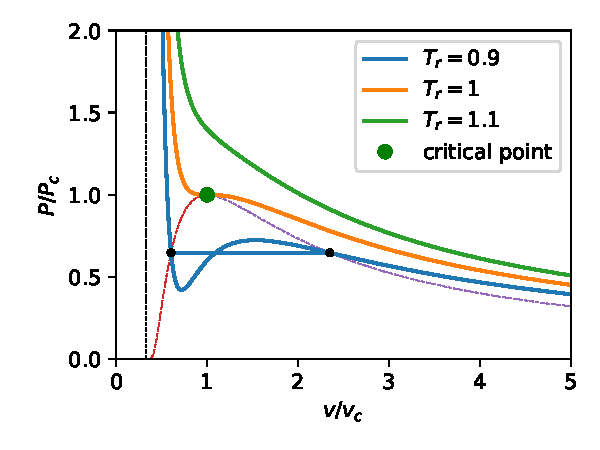
\includegraphics[scale=0.8]{figures/isotherms of the van der Waals gas.pdf}
		\caption{isotherms of the van der Waals gas.}
	\end{figure}
\end{itemize}

\subsection{critical exponents and fluctuations}
\begin{itemize}
	\item 根据 \eqref{10.2.13}, 在 critical point 附近, $T_r < 1$ 时, 有
	\begin{equation}
		v_{r, \text{liquid}} \simeq 1 - \frac{\Delta}{2}, \quad v_{r, \text{gas}} \simeq 1 + \frac{\Delta}{2},
	\end{equation}
	得到
	\begin{equation}
		T_r \simeq 1 - \frac{1}{16} (v_{r, \text{gas}} - v_{r, \text{liquid}})^2 \iff v_\text{gas} - v_\text{liquid} \sim (T_c - T)^\beta, \beta = \frac{1}{2}.
	\end{equation}
	
	\item 因为在 critical point $\big( \frac{\partial P}{\partial v} \big)_{T, N} = \big( \frac{\partial^2 P}{\partial v^2} \big)_{T, N} = 0$, 所以
	\begin{equation}
		P - P_c \sim (v - v_c)^\delta, \delta = 3 \Longrightarrow \kappa_T = - \frac{1}{v} \Big( \frac{\partial v}{\partial P} \Big)_{T, N} \sim (T - T_c)^{- \gamma}, \gamma = 1,
	\end{equation}
	可见, 在 critical point $\kappa_T \rightarrow \infty$, 根据 \eqref{4.4.2}, 直接后果就是
	\begin{equation}
		\braket{(\Delta N)^2} \rightarrow \infty.
	\end{equation}
\end{itemize}

\section{the Ising model}
\begin{itemize}
	\item 考虑一个 $D$ 维 lattice, 含有 $N$ 个 sites, 每个 lattice site 可以处于两个状态 $s_i = \pm 1$.
	
	\item 系统的能量为
	\begin{equation}
		E\{s_i\} = - B \sum_i s_i - J \sum_{\braket{i j}} s_i s_j,
	\end{equation}
	其中 $\braket{i j}$ 表示 nearest neighbor pairs.
	\begin{itemize}
		\item $J > 0$, 系统称为 ferromagnet (我们只考虑这种情况); $J < 0$, 系统称为 anti-ferromagnet.
		
		\item 用 $q$ 表示每个 lattice site 拥有的 nearest neighbors 数量, 称为 coordination number.
		
		\item $D = 1$, 那么 $q = 2$; $D = 2$ 的 square lattice, 那么 $q = 4$; $D = 2$ 的 triangular lattice, 那么 $q = 6$.
	\end{itemize}
	
	\item 系统的 partition function 为
	\begin{equation}
		Z_\text{C}(T, B, N) = \sum_{\{s_i\}} e^{- \beta E\{s_i\}}.
	\end{equation}
	
	\item 那么, 系统的 magnetization 为
	\begin{equation}
		\braket{m} \equiv \frac{1}{N} \braket{\sum_i s_i} = \frac{1}{N \beta} \frac{\partial}{\partial B} \ln Z_\text{C}(T, B, N) \equiv - \frac{1}{N} \Big( \frac{\partial F}{\partial B} \Big)_{T, N},
	\end{equation}
	并且 $m \in [- 1, 1]$.
	
	\item 分别用 $N_{\uparrow, \downarrow}$ 表示处于 $\uparrow, \downarrow$ 态的 lattice sites 数量, 以及 $N_{\braket{\uparrow \uparrow}, \braket{\uparrow \downarrow}, \braket{\downarrow \downarrow}}$ 表示三种 nearest neighbors 的数量, 那么 (可以选取 $N_\uparrow, N_{\braket{\uparrow \uparrow}}$ 为独立变量)
	\begin{equation}
		\begin{dcases}
			N_\uparrow + N_\downarrow = N \\
			q N_\uparrow = 2 N_{\braket{\uparrow \uparrow}} + N_{\braket{\uparrow \downarrow}} \\
			q N_\downarrow = 2 N_{\braket{\downarrow \downarrow}} + N_{\braket{\uparrow \downarrow}}
		\end{dcases} \Longrightarrow N_{\braket{\cdot \cdot}} = \frac{q}{2} N,
	\end{equation}
	以及
	\begin{equation}
		\begin{dcases}
			E(N_\uparrow, N_{\braket{\uparrow \uparrow}}) = - B (2 N_\uparrow - N) - J \Big( \frac{q}{2} N - 2 q N_\uparrow + 4 N_{\braket{\uparrow \uparrow}} \Big) \\
			m = 2 \frac{N_\uparrow}{N} - 1
		\end{dcases}.
	\end{equation}
\end{itemize}

\subsection{mean field theory}
\begin{itemize}
	\item 假设 lattice site 处于 spin-up 和 spin-down 的概率与其 nearest neighbor 的状态无关, 那么
	\begin{equation}
		N_{\braket{\uparrow \downarrow}} \approx N_{\braket{\cdot \cdot}} \Big( \frac{N_\uparrow}{N} \frac{N_\downarrow}{N} + \frac{N_\downarrow}{N} \frac{N_\uparrow}{N} \Big) = q \frac{N_\uparrow N_\downarrow}{N},
	\end{equation}
	等价于
	\begin{equation}
		\sum_{\braket{i j}} (s_i - m) (s_j - m) \approx 0 \quad \text{or} \quad N_{\braket{\uparrow \uparrow}} \approx \frac{q}{2} \frac{N_\uparrow^2}{N}.
	\end{equation}
	
	\item 那么
	\begin{equation}
		\begin{dcases}
			E_\text{mf} = N \Big( - B m - \frac{q}{2} J m^2 \Big) = N \Big( - B_\text{eff} m + \frac{q}{2} J m^2 \Big) \\
			\Omega(m) = \frac{N!}{N_\uparrow! N_\downarrow!} \simeq \exp \Big( N \Big( \ln 2 - \frac{1 + m}{2} \ln(1 + m) - \frac{1 - m}{2} \ln(1 - m) \Big) \Big) \leq 2^N
		\end{dcases},
	\end{equation}
	其中 $B_\text{eff}(m) = B + q J m$ 称为 mean field. 因此
	\begin{align}
		\ln Z_\text{C,mf} &\simeq \max(\ln \Omega(m) - \beta E_\text{mf}(m)) \notag \\
		&= N \Big( \ln(2 \cosh \beta B_\text{eff}(m_0)) - \beta \frac{q}{2} J m_0^2 \Big),
	\end{align}
	得到
	\begin{equation}
		\braket{m} \simeq m_0 = \tanh(\beta B_\text{eff}(m_0)),
	\end{equation}
	其中 $m_0$ 为 global maximum point.
	
	\begin{tcolorbox}[title=calculation:]
		\begin{equation}
			0 = \frac{1}{N} \frac{\partial}{\partial m} (\ln \Omega(m) - \beta E_\text{mf}(m)) = \frac{1}{2} \ln \frac{1 - m}{1 + m} + \beta (B + q J m).
		\end{equation}
	\end{tcolorbox}
	
	\item 得到 $T$--$m_0$ 关系如下图:
	
	\begin{figure}[H]
		\centering
		\begin{subfigure}{0.4\linewidth}
			\centering
			\includegraphics[scale=0.8]{figures/plot of T--m_0 with frac{B}{qJ}=0.pdf}
			\caption{plot of $T$--$m_0$ with $\frac{B}{qJ} = 0$.}
		\end{subfigure}
		\begin{subfigure}{0.4\linewidth}
			\centering
			\includegraphics[scale=0.8]{figures/plot of T--m_0 with frac{B}{qJ}=0.05.pdf}
			\caption{plot of $T$--$m_0$ with $\frac{B}{qJ} = 0.05$.}
			\label{figure 10.2 (b)}
		\end{subfigure}
		\caption{}
	\end{figure}
	
	\begin{itemize}
		\item figure \ref{figure 10.2 (b)} 中, 蓝色曲线对应 global maximum, 而橙色曲线只是 local maximum, 舍去.
		
		\item $B = 0$ 时, 系统在
		\begin{equation}
			k_B T_c = q J
		\end{equation}
		发生相变.
	\end{itemize}
\end{itemize}

\subsection{critical exponents}
\begin{itemize}
	\item $B = 0$, 在 $T \rightarrow T_c + 0^-$ 附近 $|m_0| \ll 1$, 那么
	\begin{equation}
		m_0(B = 0) \simeq \pm \sqrt{\frac{3}{T_c}} (T_c - T)^\beta, \beta = \frac{1}{2}.
	\end{equation}
	
	\item $T = T_c$, 在 $B \rightarrow 0$ 附近 $|m_0| \ll 1$, 那么
	\begin{equation}
		m_0(T = T_c) \simeq \Big( 3 \frac{B}{k_B T_c} \Big)^{\frac{1}{\delta}}, \delta = 3.
	\end{equation}
	
	\item 类比 $\kappa_T$, 计算 susceptibility,
	\begin{equation}
		\chi = \Big( \frac{\partial \braket{m}}{\partial B} \Big)_{T, N} = \frac{\beta}{\cosh^2 \beta B_\text{eff}} \Big( 1 - \frac{\beta q J}{\cosh^2 \beta B_\text{eff}} \Big)^{- 1},
	\end{equation}
	当 $B = 0, T \rightarrow T_c + 0^-$ 时, 有 $\beta B_\text{eff} \simeq \sqrt{\frac{3}{T_c}} (T_c - T)^{1 / 2}$, 所以
	\begin{equation}
		\chi \simeq \frac{1}{4 k_B} (T_c - T)^{- \gamma}, \gamma = 1.
	\end{equation}
	
	\item mean field theory 得到的 critical exponents 和 van der Waals equation 的一样, 为 $\beta = \frac{1}{2}, \delta = 3, \gamma = 1$.
\end{itemize}

\section{some exact results for the Ising model}
\subsection{the Ising model in \texorpdfstring{$D = 1$}{D=1} dimensions}
\begin{itemize}
	\item $D = 1$ Ising model 也称为 Ising chain, 具有循环边界条件 $s_i = s_{N + 1}$, 那么
	\begin{equation} \label{11.4.1}
		Z_\text{C}(T, B, N) = \sum_{s_1 = \pm 1} \cdots \sum_{s_N = \pm 1} \prod_{i = 1}^N \exp(\beta B s_i + \beta J s_i s_{i + 1}) = \lambda_+^N + \lambda_-^N \simeq \lambda_+^N,
	\end{equation}
	其中
	\begin{equation}
		\lambda_\pm = e^{\beta J} \cosh \beta B \pm \sqrt{e^{2 \beta J} \cosh^2 \beta B - 2 \sinh 2 \beta J}.
	\end{equation}
	
	\begin{tcolorbox}[title=calculation:]
		对 $Z_\text{C}$ 稍作改写
		\begin{equation}
			Z_\text{C}(T, B, N) = \sum_{s_1 = \pm 1} \cdots \sum_{s_N = \pm 1} \prod_{i = 1}^N \exp \Big( \frac{1}{2} \beta B (s_i + s_{i + 1}) + \beta J s_i s_{i + 1} \Big),
		\end{equation}
		注意到
		\begin{equation}
			\exp \Big( \frac{1}{2} \beta B (s_i + s_{i + 1}) + \beta J s_i s_{i + 1} \Big) = \braket{s_i | \begin{pmatrix}
				e^{\beta B + \beta J} & e^{- \beta J} \\
				e^{- \beta J} & e^{- \beta B + \beta J}
			\end{pmatrix} | s_{i + 1}},
		\end{equation}
		其中
		\begin{equation}
			\ket{1} = \begin{pmatrix}
				1 \\
				0
			\end{pmatrix}, \quad \ket{- 1} = \begin{pmatrix}
				0 \\
				1
			\end{pmatrix},
		\end{equation}
		因此
		\begin{equation}
			Z_\text{C}(T, B, N) = \mathrm{Tr} \begin{pmatrix}
				e^{\beta B + \beta J} & e^{- \beta J} \\
				e^{- \beta J} & e^{- \beta B + \beta J}
			\end{pmatrix}^N = \cdots
		\end{equation}
	\end{tcolorbox}
	
	\begin{itemize}
		\item $\lambda_\pm(T, B)$ 的函数图像如下:
		
		\begin{figure}[H]
			\centering
			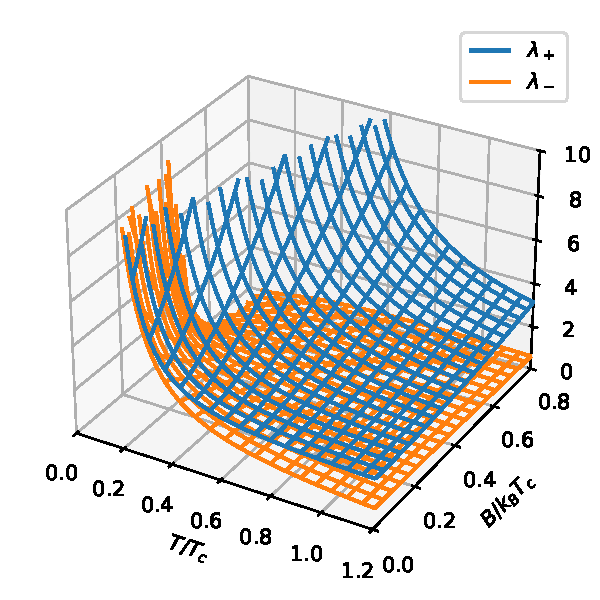
\includegraphics[scale=0.8]{figures/plot of lambda_+ and lambda_-.pdf}
			\caption{plot of $\lambda_\pm(T, B)$.}
		\end{figure}
		
		\item 注意到
		\begin{equation}
			\lambda_-(T \rightarrow 0, B) = e^{\beta (J - B)} = \begin{dcases}
				\infty & B < J \\
				1 & B = J \\
				0 & B > J
			\end{dcases}.
		\end{equation}
	\end{itemize}
	
	\item 得到
	\begin{equation}
		\braket{m} = \frac{1}{N \beta} \frac{\partial}{\partial B} \ln Z_\text{C} = \frac{e^{\beta J} \sinh \beta B}{\sqrt{e^{2 \beta J} \cosh^2 \beta B - 2 \sinh 2 \beta J}},
	\end{equation}
	并注意到
	\begin{equation}
		\braket{m}(T, B = 0) = 0.
	\end{equation}
	
	\item $\braket{m}(T, B)$ 的函数图像如下:
	
	\begin{figure}[H]
		\centering
		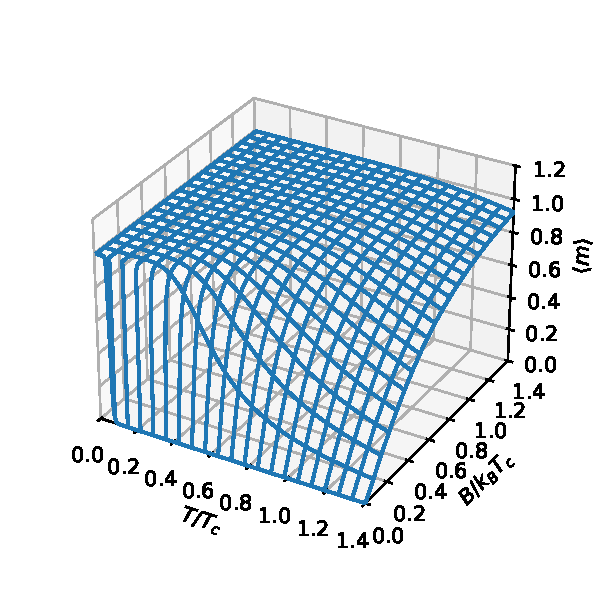
\includegraphics[scale=0.8]{figures/plot of the magnetization.pdf}
		\caption{plot of the magnetization.}
	\end{figure}
	
	\item 可见, Ising chain 中不存在 phase transition, 与 mean field theory 预测的结果完全不同.
\end{itemize}

\subsection{2-dim. Ising model: low temperatures and Peierls droplets}
\begin{itemize}
	\item 考虑 $B = 0, T \rightarrow 0$ 下的 2-dim. square lattice.
	
	\item 2-dim. Ising model 的最低 3 个能级如下图所示:
	
	\begin{figure}[H]
		\centering
		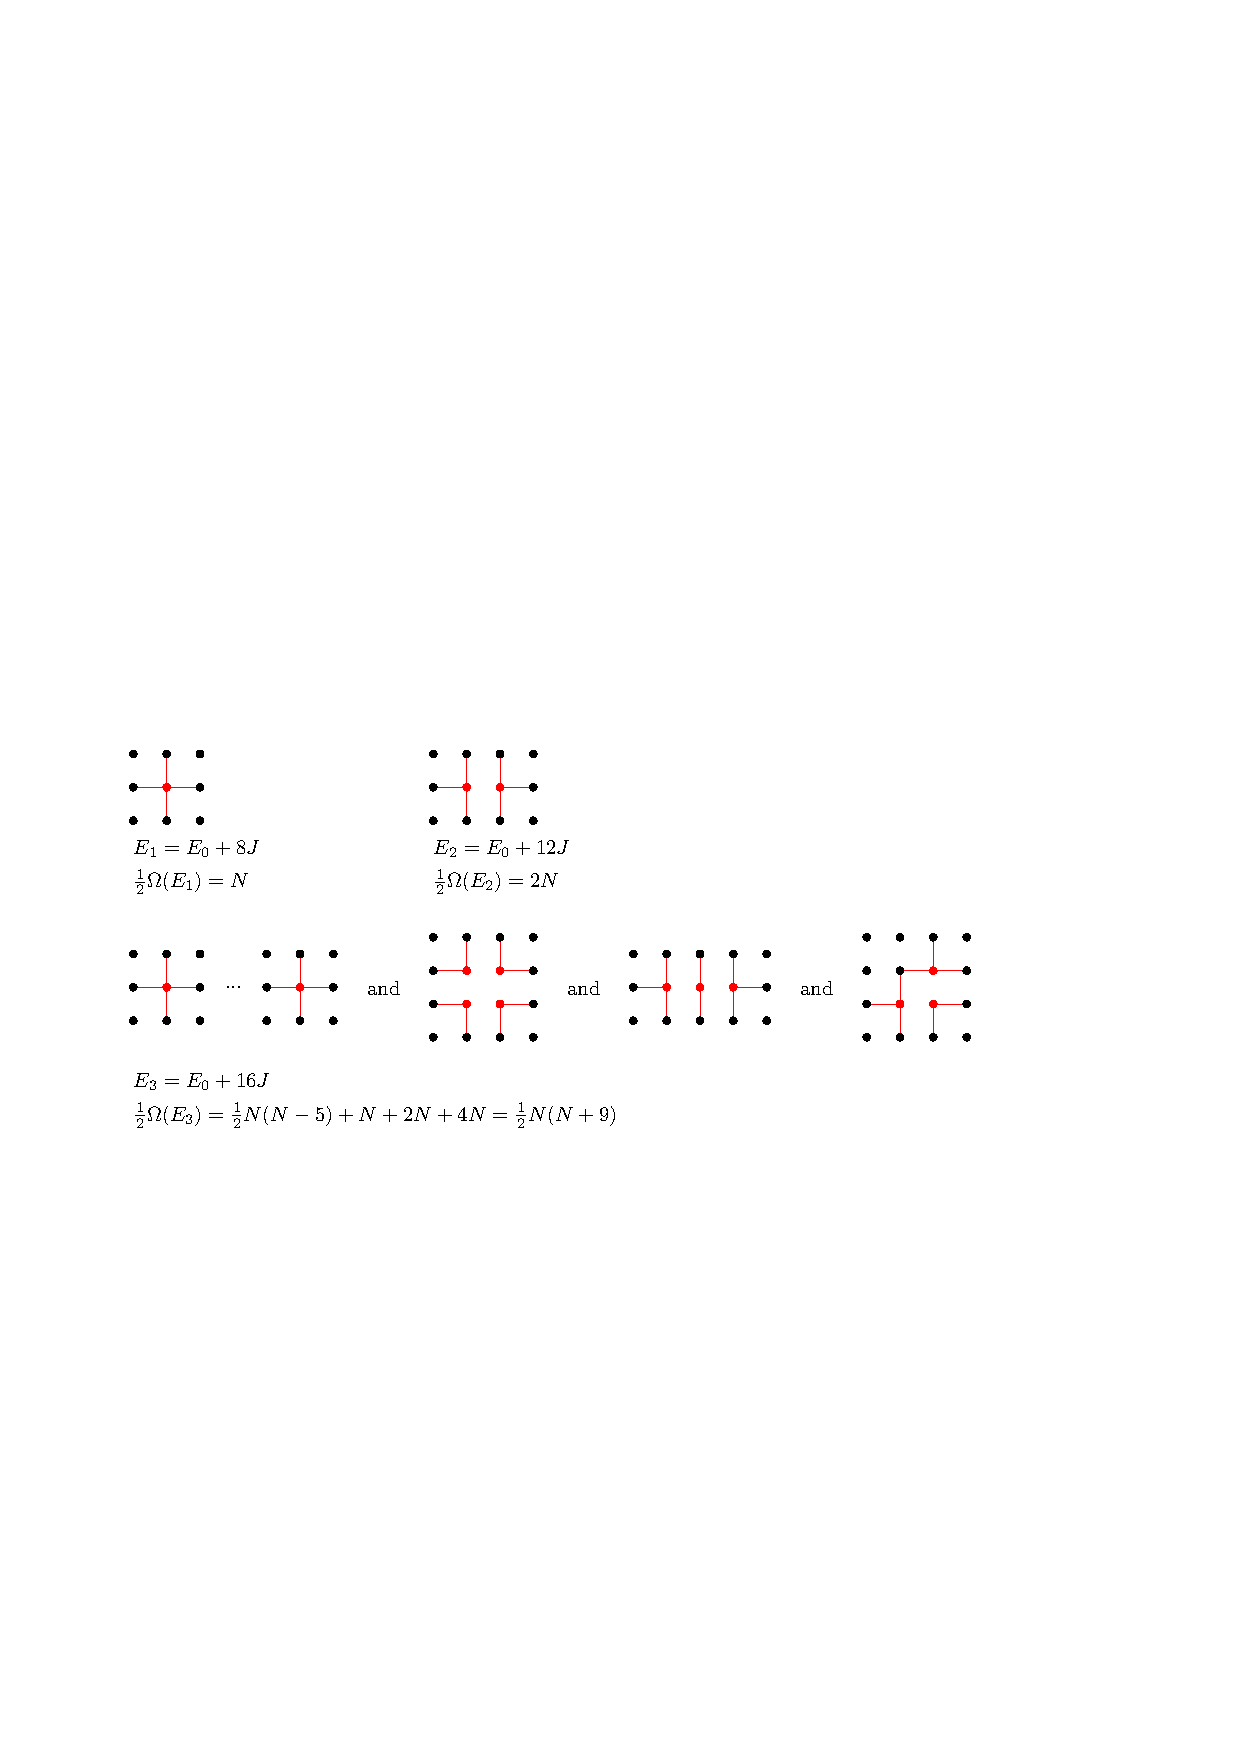
\includegraphics[scale=1]{figures/lowest 3 energy levels of the 2-dim. Ising model.pdf}
		\caption{lowest 3 energy levels of the 2-dim. Ising model.}
	\end{figure}
	
	\item 因此, 低温下近似有
	\begin{equation} \label{11.4.10}
		Z_\text{C} = 2 e^{- \beta E_0} \Big( 1 + N e^{- 8 \beta J} + 2 N e^{- 12 \beta J} + \frac{1}{2} N (N + 9) e^{- 16 \beta J} + \cdots \Big),
	\end{equation}
	其中 $E_0 = - 2 N J$, 并注意到 $\Omega(E_0) = 2$.
	
	\item 系统的 Helmholtz free energy 为 (注意 $\ln(1 + x) = x - \frac{x^2}{2} + \cdots$)
	\begin{align}
		- \beta F &= \ln Z_\text{C} \notag \\
		&= \ln 2 + 2 N \beta J + \Big( N e^{- 8 \beta J} + 2 N e^{- 12 \beta J} + \frac{1}{2} N (N + 9) e^{- 16 \beta J} + \cdots \Big) - \frac{1}{2} N^2 e^{- 16 \beta J} + \cdots \notag \\
		&= \ln 2 + 2 N \beta J + \Big( N e^{- 8 \beta J} + 2 N e^{- 12 \beta J} + \frac{9}{2} N e^{- 16 \beta J} + \cdots \Big),
	\end{align}
	可见 $F \propto N$.
	\begin{itemize}
		\item general lesson: partition function can be written as the exponential of the sum of \textbf{connected diagrams}.
	\end{itemize}
	
	\item 系统的 magnetization 为 (注意 $\frac{1}{1 + x} = 1 - x + x^2 + \cdots$)
	\begin{align}
		\braket{m} =& \pm \frac{2}{Z_\text{C}} e^{- \beta E_0} \bigg( 1 + \Big( 1 - \frac{2}{N} \Big) N e^{- 8 \beta J} + \Big( 1 - \frac{4}{N} \Big) 2 N e^{- 12 \beta J} \notag \\
		& + \Big( \Big( 1 - \frac{4}{N} \Big) \frac{1}{2} N (N - 5) + \Big( 1 - \frac{8}{N} \Big) N + \Big( 1 - \frac{6}{N} \Big) 2 N + \Big( 1 - \frac{6}{N} \Big) 4 N \Big) e^{- 16 \beta J} + \cdots \bigg) \notag \\
		=& \pm (1 - 2 e^{- 8 \beta J} - 8 e^{- 12 \beta J} - 34 e^{- 16 \beta J} - \cdots).
	\end{align}
\end{itemize}

\subsubsection{Peierls droplets}
\begin{itemize}
	\item 当温度升高时, low energy states become droplets, 对于一个周长为 $L$ 的 droplet, 其能量为
	\begin{equation}
		E \sim 2 J L,
	\end{equation}
	其 degeneracy (用 random walk 估计) 为
	\begin{equation}
		\Omega \sim e^{\alpha L},
	\end{equation}
	其中 $\ln 2 < \alpha < \ln 3$.
	
	\item 系统的 partition function 为
	\begin{equation}
		Z \sim \sum_L e^{(\alpha - 2 \beta J) L},
	\end{equation}
	估计相变发生在 $E \sim T_c S$, 因此
	\begin{equation} \label{11.4.16}
		k_B T_c \sim \frac{2 J}{\alpha}.
	\end{equation}
	
	\noindent\rule[0.5ex]{\linewidth}{0.5pt} % horizontal line
	
	\item 对于 $D = 1$ 的情况, droplet 的能量为
	\begin{equation}
		E = 2 J,
	\end{equation}
	其 degeneracy 为
	\begin{equation}
		\Omega = N,
	\end{equation}
	那么
	\begin{equation}
		Z \sim N e^{- \beta 2 J}
	\end{equation}
	可见相变温度估计为
	\begin{equation}
		T_c \sim \frac{2 J}{\ln N} \simeq 0,
	\end{equation}
	因此, 任何温度下 entropy 都占主导, $\braket{m} = 0$.
\end{itemize}

\subsection{2-dim. Ising model: high temperatures}
\begin{itemize}
	\item 考虑 $B = 0, \beta J \ll 1$ 下的 2-dim. square lattice.
	
	\item 注意到 $s_i s_j = \pm 1$, 因此
	\begin{equation}
		e^{\beta J s_i s_j} = \cosh \beta J + s_i s_j \sinh \beta J = \begin{dcases}
			e^{\beta J} & s_i s_j = + 1 \\
			e^{- \beta J} & s_i s_j = - 1
		\end{dcases},
	\end{equation}
	所以
	\begin{equation}
		Z_\text{C} = \sum_{\{s_i\}} \prod_{\braket{i j}} e^{\beta J s_i s_j} = \cosh^{q N / 2} \beta J \sum_{\{s_i\}} \prod_{\braket{i j}} (1 + s_i s_j \tanh \beta J).
	\end{equation}
	
	\item 对求和中的 $\tanh \beta J$ 作展开, 得到
	\begin{equation} \label{11.4.23}
		Z_\text{C} = 2^N \cosh^{2 N} \beta J \Big( 1 + N \tanh^4 \beta J + 2 N \tanh^6 \beta J + \frac{1}{2} N (N + 9) \tanh^8 \beta J + \cdots \Big).
	\end{equation}
	
	\begin{tcolorbox}[title=calculation:]
		\begin{align}
			& \sum_{\{s_i\}} \prod_{\braket{i j}} (1 + s_i s_j \tanh \beta J) \notag \\
			=& 2^N + \sum_{\{s_i\}} \sum_{\braket{i j}} s_i s_j \tanh \beta J + \frac{1}{2} \sum_{\{s_i\}} \sum_{\braket{i j} \neq \braket{k l}} s_i s_j s_k s_l \tanh^2 \beta J \notag \\
			& + \frac{1}{3!} \sum_{\{s_i\}} \sum_{\braket{i j} \neq \braket{k l} \neq \braket{m n}} \cdots,
		\end{align}
		但是, 注意到
		\begin{equation}
			\vcenter{\hbox{
\includegraphics[scale=1]{figures/graph of s_i s_j.pdf}}} = \sum_{s_i, s_j = \pm 1} s_i s_j = + 1 - 1 - 1 + 1 = 0,
		\end{equation}
		要避免求和为零, 就必须让每一个 lattice site 都是平方项, 比如 (注意, 下图中 $1, 4$ 不是 nearest neighbor)
		\begin{equation} \label{11.4.26}
			\vcenter{\hbox{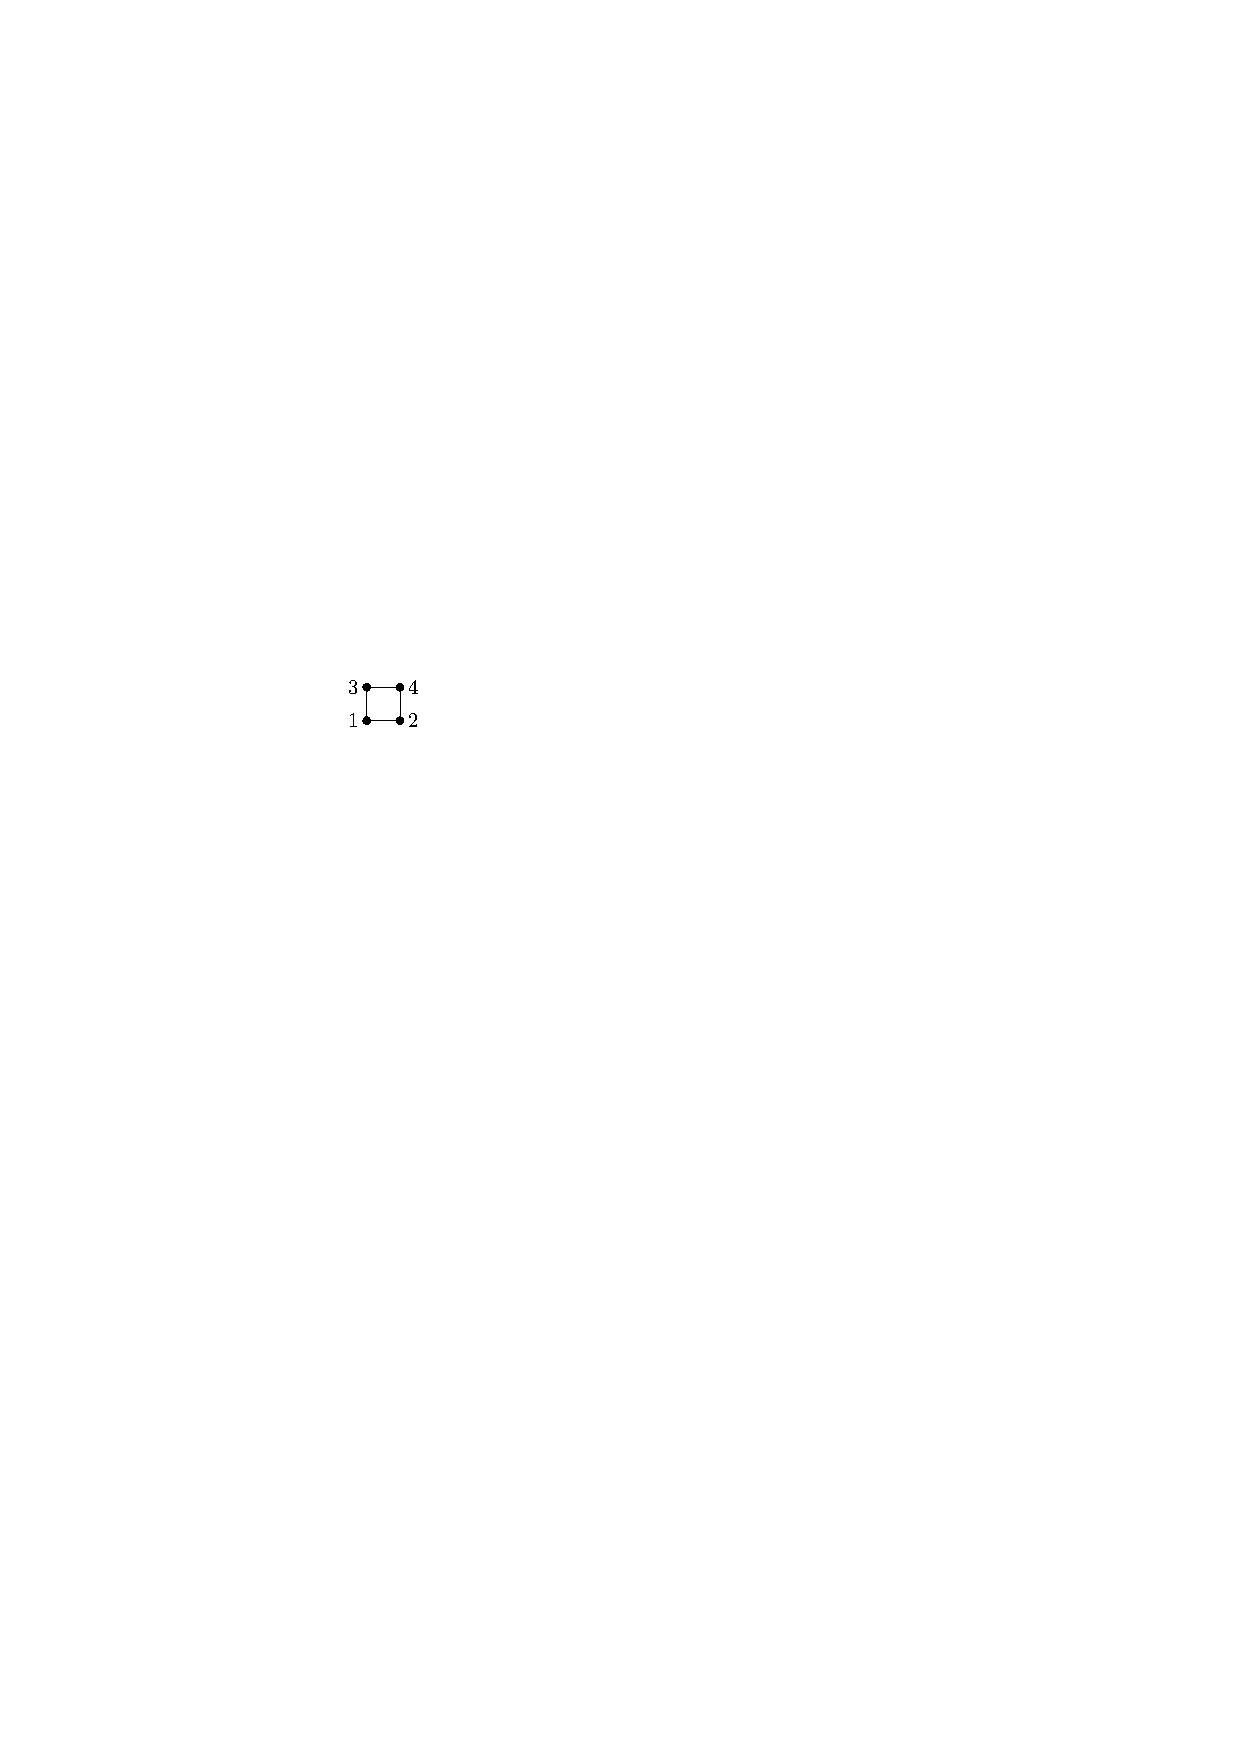
\includegraphics[scale=1]{figures/graph of (s_1 s_2 s_3 s_4)^2.pdf}}} = \sum (s_1 s_2) (s_2 s_4) (s_4 s_3) (s_3 s_1) = 2^4,
		\end{equation}
		因此
		\begin{equation}
			\text{sum} = 2^N + N \underbrace{2^{N - 4} 2^4}_{= 2^N} \tanh^4 \beta J + \cdots,
		\end{equation}
		类似地, 6 阶和 8 阶修正分别为
		\begin{equation}
			\begin{dcases}
				\vcenter{\hbox{
\includegraphics[scale=1]{figures/graph of the 6th order terms (1).pdf}}} + \vcenter{\hbox{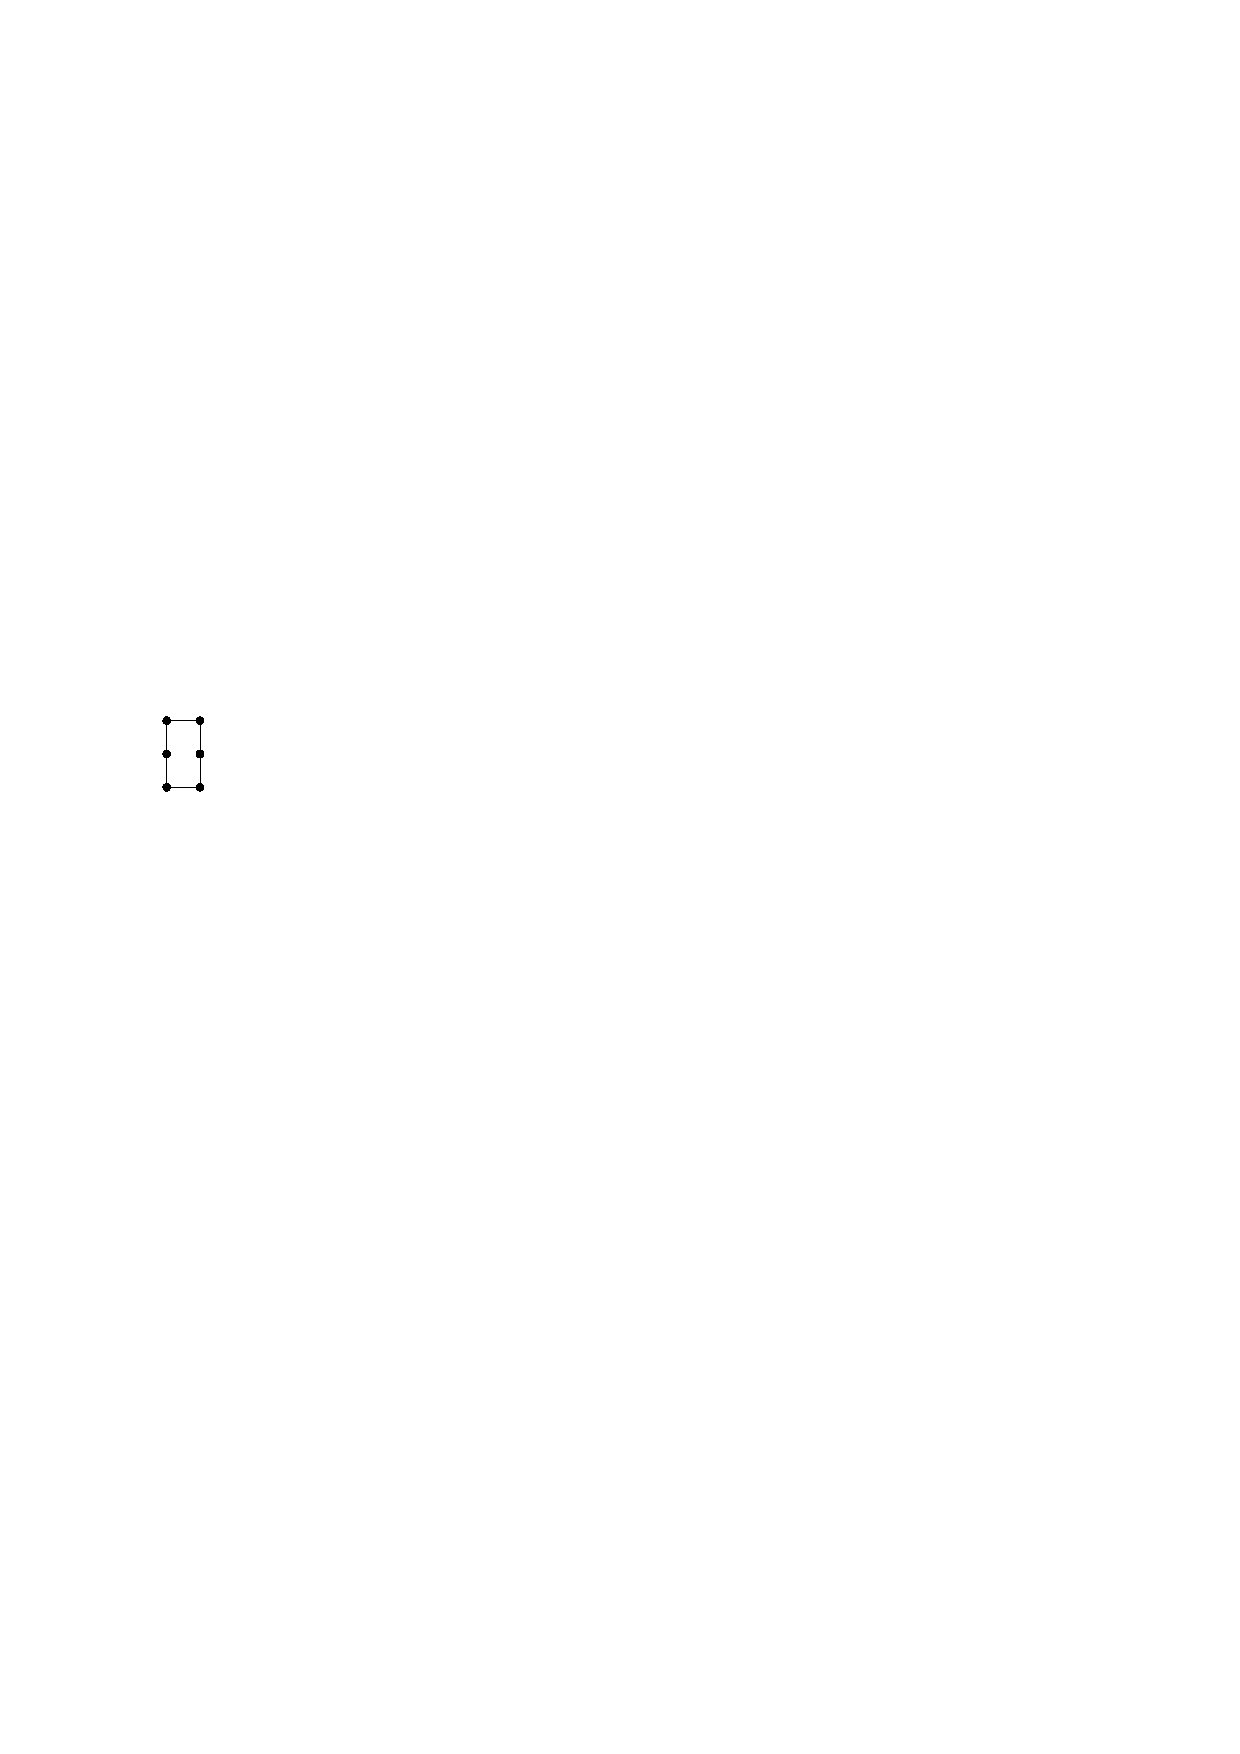
\includegraphics[scale=1]{figures/graph of the 6th order terms (2).pdf}}} = 2 N 2^N \tanh^6 \beta J \\
				\begin{aligned}
					& \vcenter{\hbox{
\includegraphics[scale=1]{figures/graph of the 8th order terms (1).pdf}}} + \vcenter{\hbox{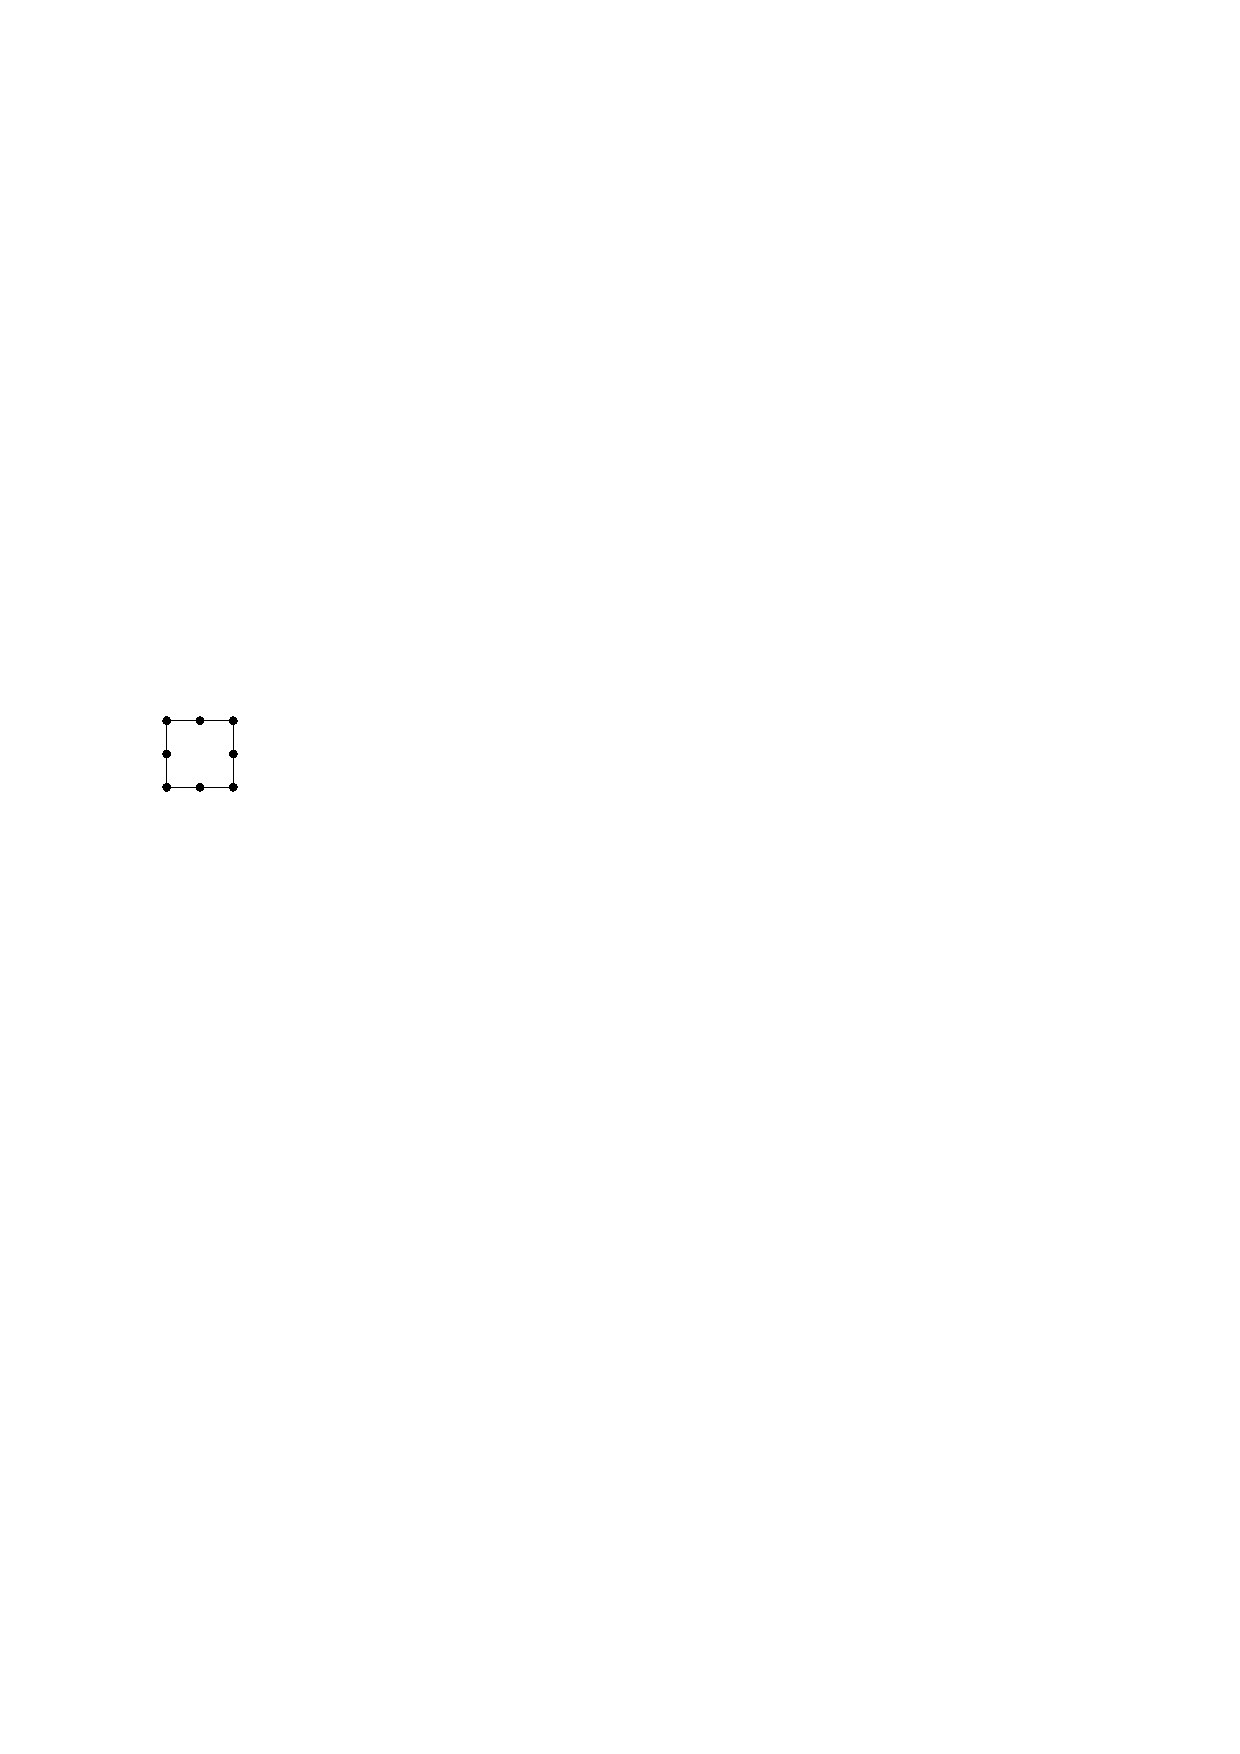
\includegraphics[scale=1]{figures/graph of the 8th order terms (2).pdf}}} + \vcenter{\hbox{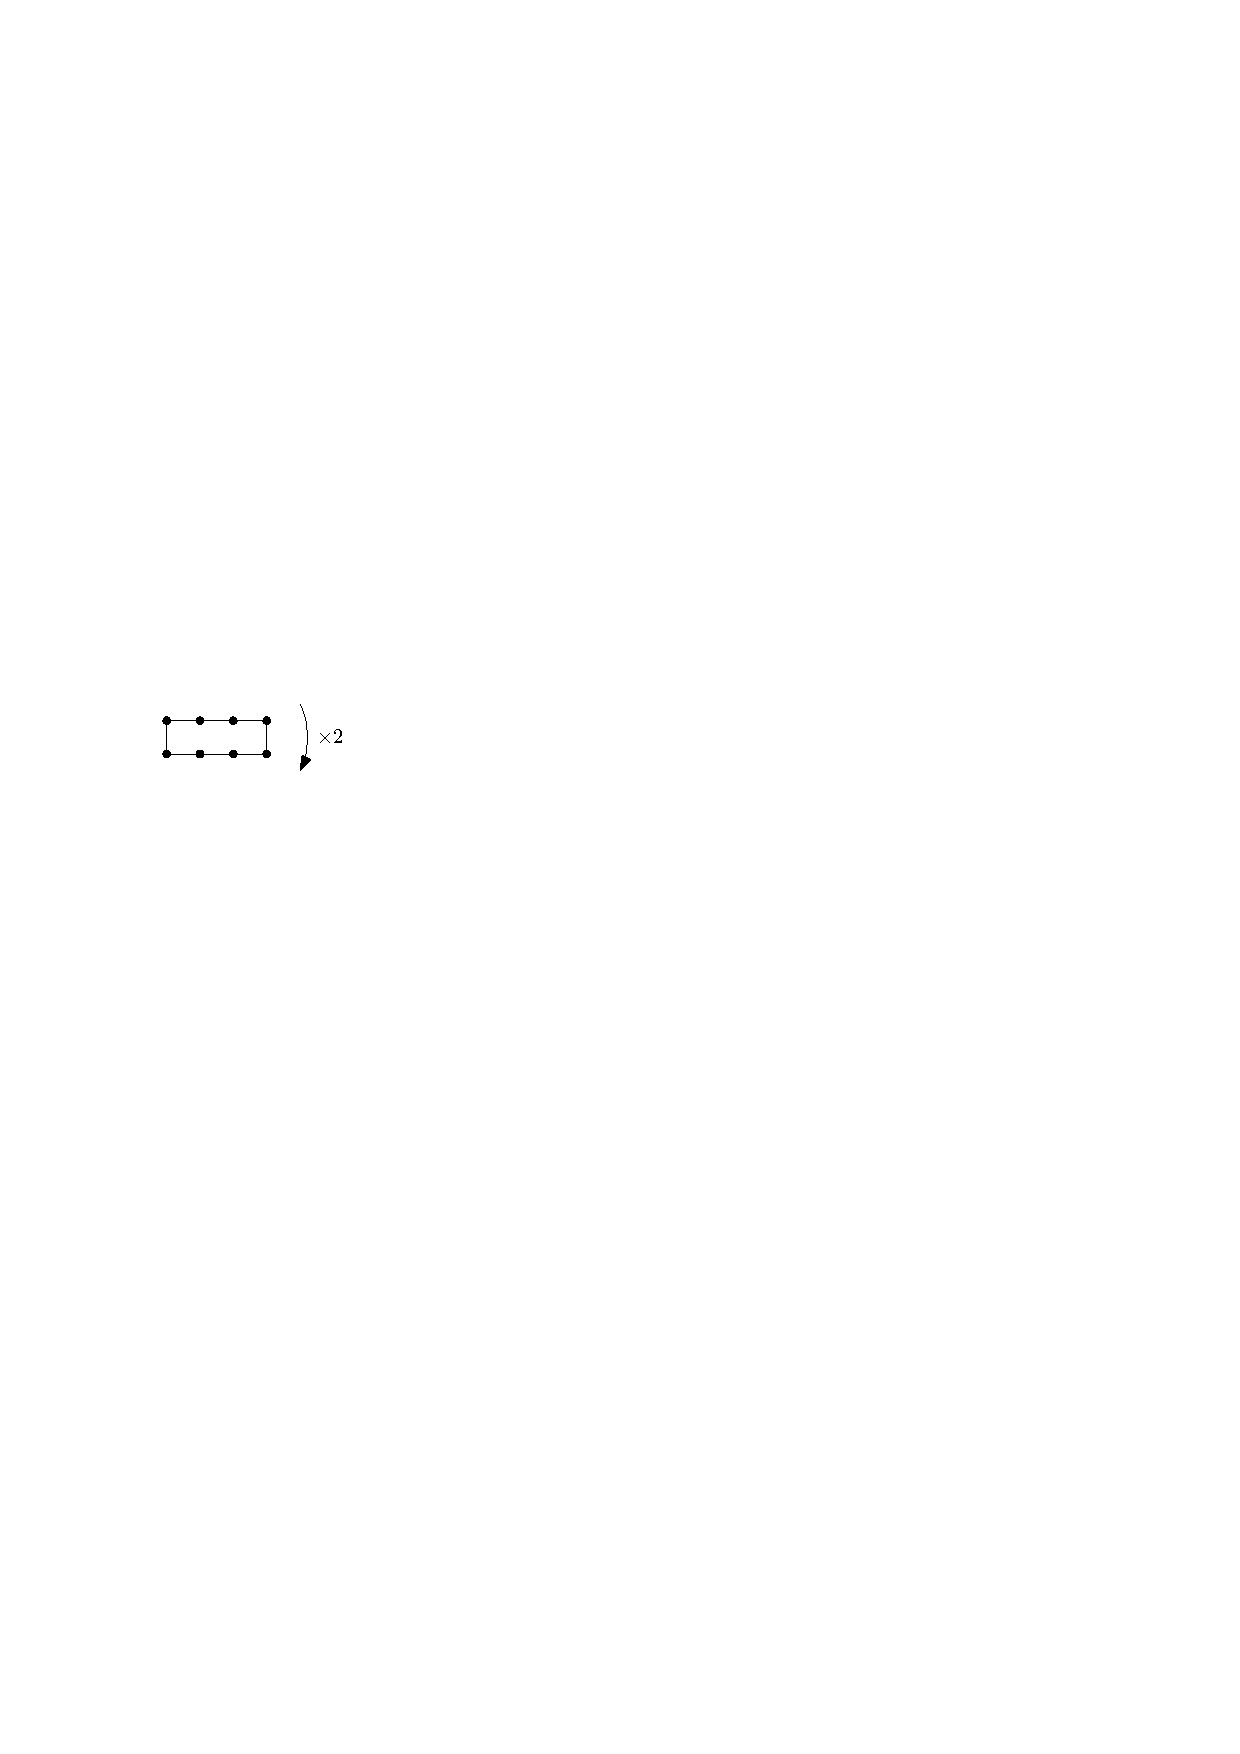
\includegraphics[scale=1]{figures/graph of the 8th order terms (3).pdf}}} + \vcenter{\hbox{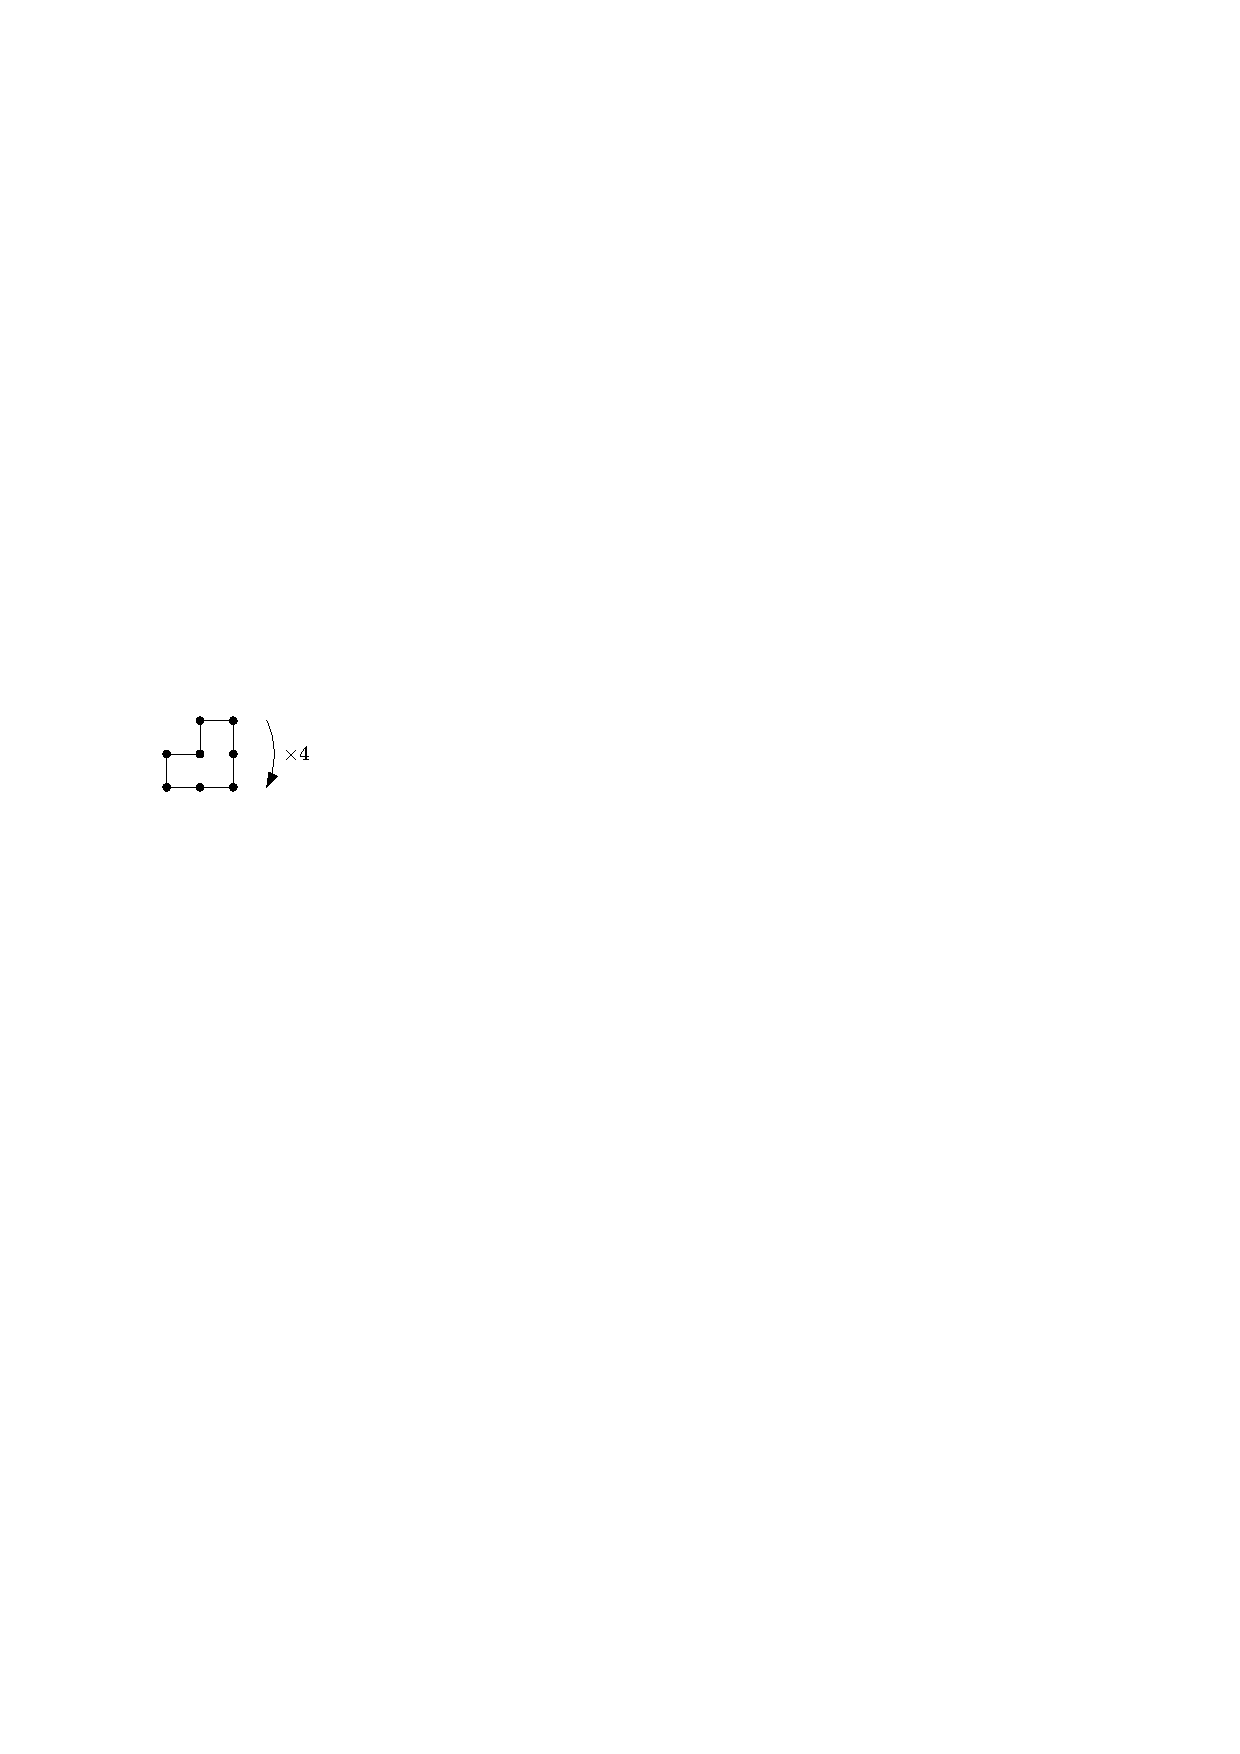
\includegraphics[scale=1]{figures/graph of the 8th order terms (4).pdf}}} \\
					&= \Big( \frac{1}{2} N (N - 5) + N + 4 N + 2 N \Big) 2^N \tanh^8 \beta J
				\end{aligned}
			\end{dcases},
		\end{equation}
		因此
		\begin{equation}
			\text{sum} = 2^N \Big( 1 + N \tanh^4 \beta J + 2 N \tanh^6 \beta J + \frac{1}{2} N (N + 9) \tanh^8 \beta J + \cdots \Big).
		\end{equation}
	\end{tcolorbox}
\end{itemize}

\subsubsection{high temperature expansion in the Ising chain}
\begin{itemize}
	\item 在 1-dim. 情况下, 显然不存在类似 \eqref{11.4.26} 的闭环, 因此
	\begin{align}
		Z_\text{C} &= \cosh^N \beta J \Big( 2^N + \vcenter{\hbox{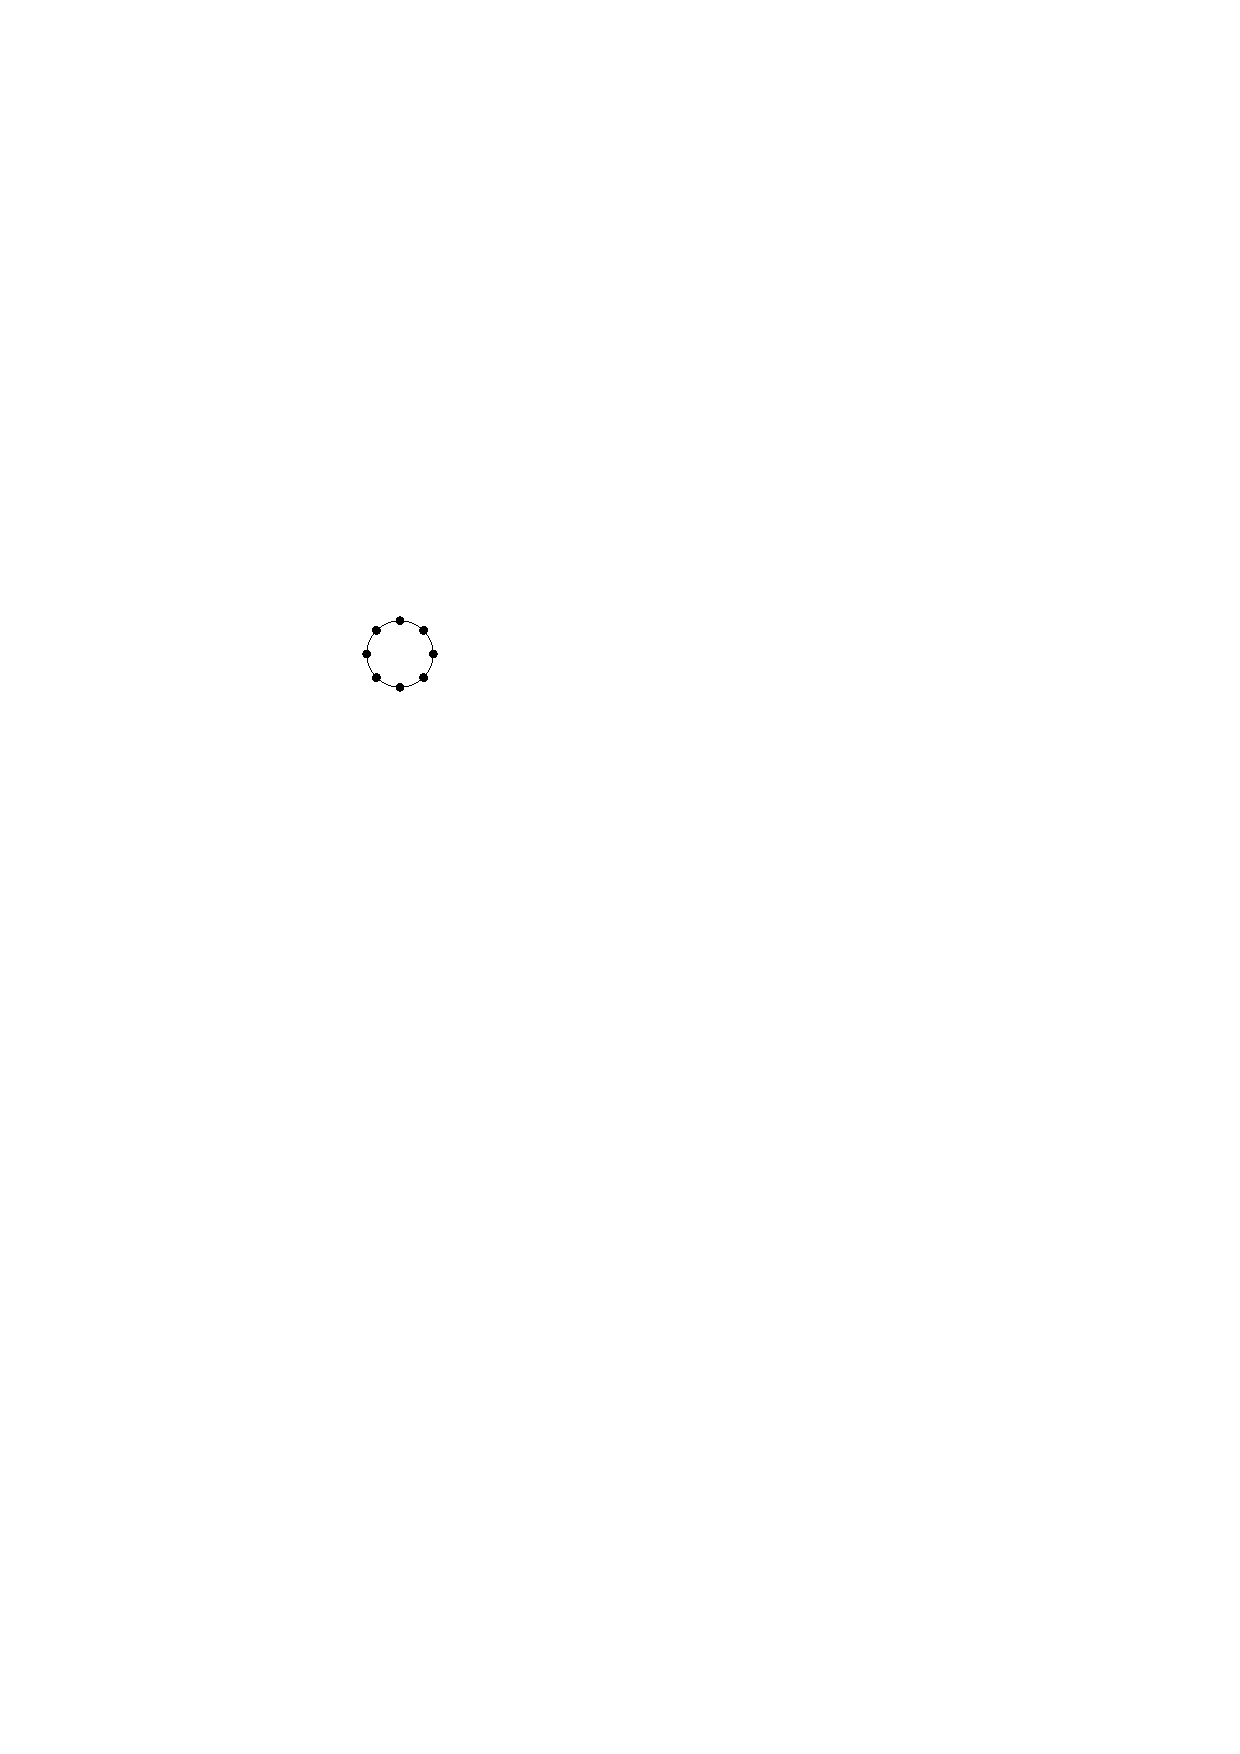
\includegraphics[scale=1]{figures/graph of the Nth order term in the Ising chain.pdf}}} \Big) \notag \\
		&= 2^N \cosh^N \beta J (1 + \tanh^N \beta J) = (2 \cosh \beta J)^N + (2 \sinh \beta J)^N \simeq (2 \cosh \beta J)^N,
	\end{align}
	对比 \eqref{11.4.1}, 并注意到 $\lambda_+(B = 0) = 2 \cosh \beta J, \lambda_-(B = 0) = 2 \sinh \beta J$, 完全符合之前的计算.
\end{itemize}

\subsection{Kramers--Wannier duality}
\begin{itemize}
	\item 对比 \eqref{11.4.10} 和 \eqref{11.4.23}, 低温和高温极限下的 partition function 有对应关系, 只需要作代换
	\begin{equation}
		e^{- 2 \beta J} \leftrightarrow \tanh \beta J
	\end{equation}
	两式就完全一样了, 这种对称性称为 Kramers--Wannier duality.
	
	\item Kramers--Wannier duality 源于低温和高温极限下计算中的 graphs are dual, 如下图所示:
	
	\begin{figure}[H]
		\centering
		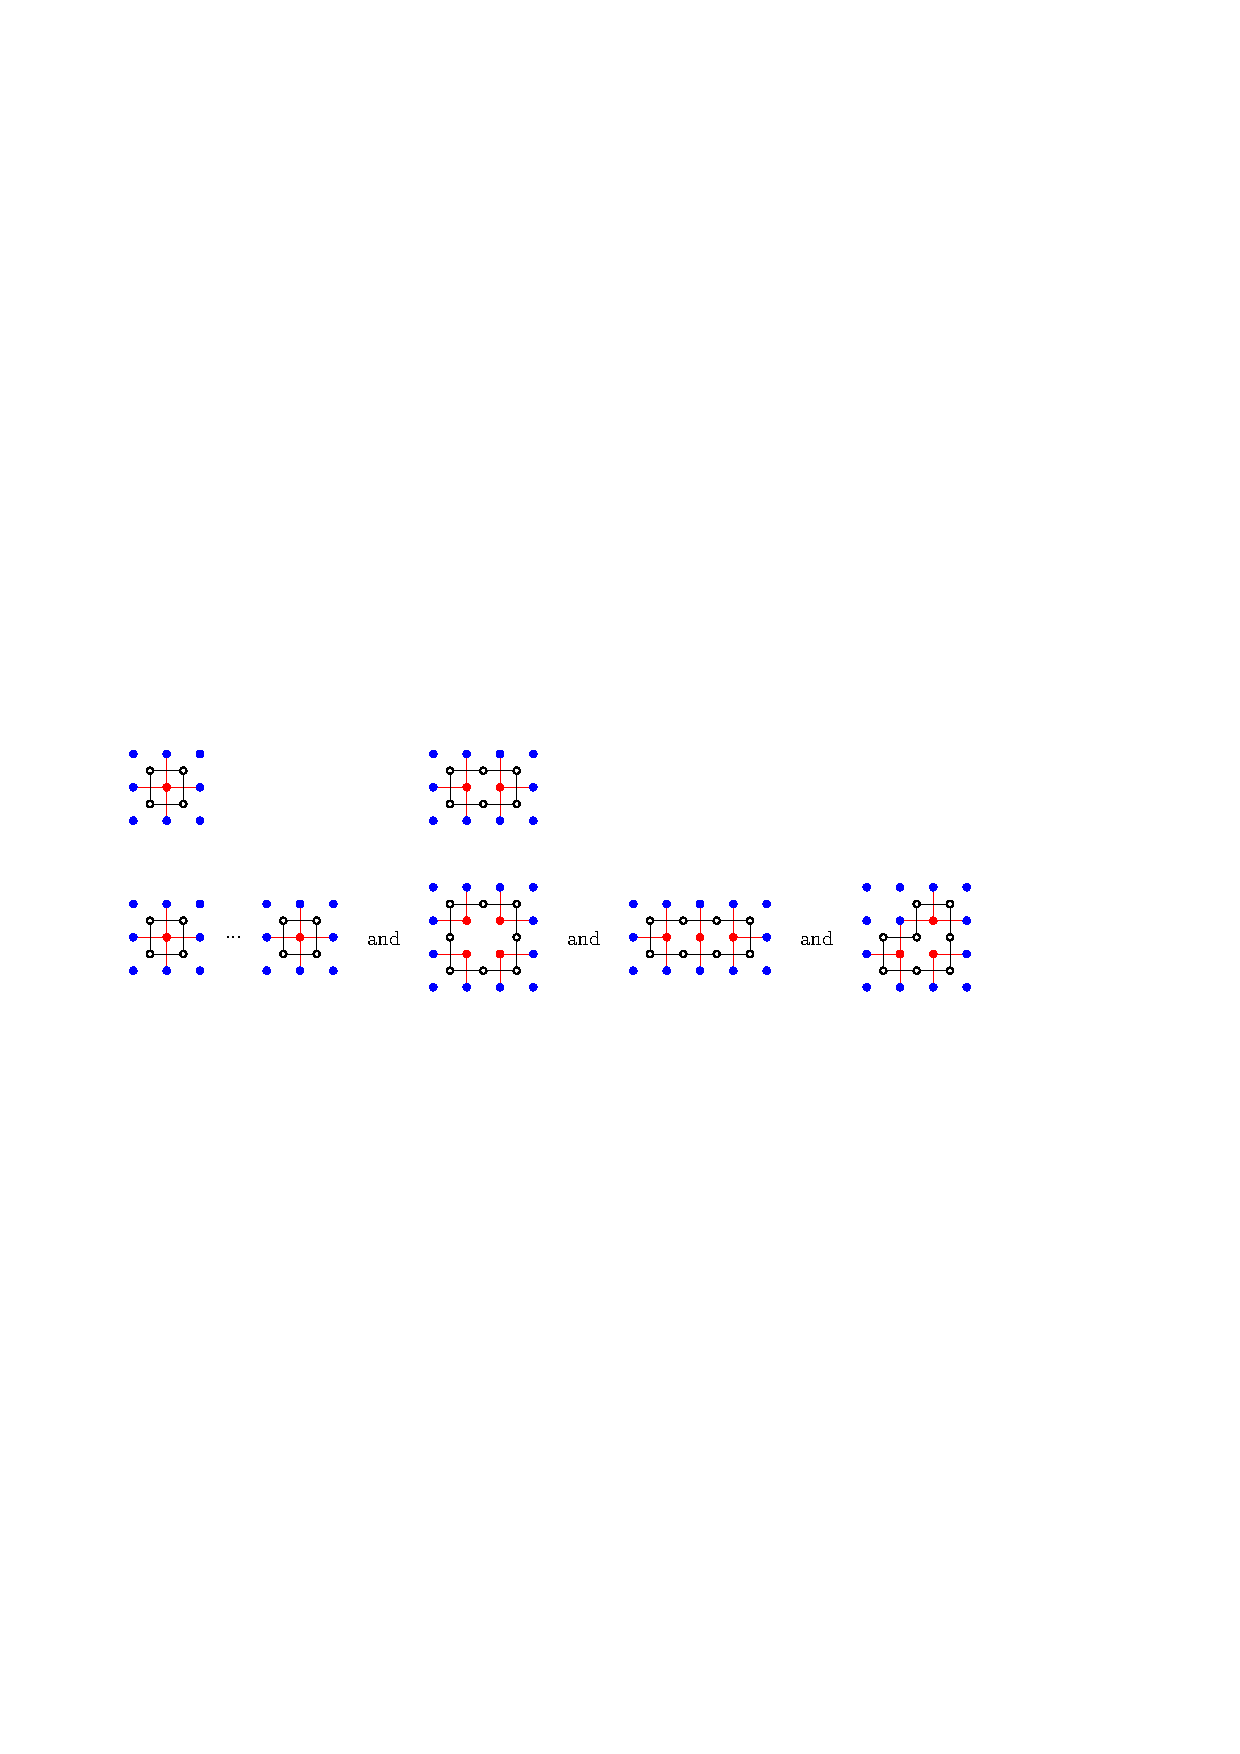
\includegraphics[scale=1]{figures/Kramers--Wannier duality.pdf}
		\caption{Kramers--Wannier duality.}
	\end{figure}
	
	\item 更准确地表述 duality 为
	\begin{equation}
		e^{- 2 \tilde{\beta} J} = \tanh \beta J \Longrightarrow \sinh 2 \tilde{\beta} J = \frac{1}{\sinh 2 \beta J},
	\end{equation}
	其中 $\tilde{\beta} J \gg 1, \beta J \ll 1$, 那么
	\begin{equation}
		Z_\text{C}(\beta) = \frac{2^N \cosh^{2 N} \beta J}{2 e^{- \tilde{\beta} E_0}} Z_\text{C}(\tilde{\beta}) = \frac{1}{2 \sinh^N 2 \tilde{\beta} J} Z_\text{C}(\tilde{\beta}).
	\end{equation}
	
	\item 相变发生在 self-dual point $\tilde{\beta} = \beta$, 得到 critical temperature 为
	\begin{equation}
		k_B T_c = \frac{2 J}{\ln(\sqrt{2} + 1)} \approx 2.269 J,
	\end{equation}
	与 Peierls droplet 的估计 \eqref{11.4.16} 相符.
\end{itemize}

\section{Landau theory}
\begin{itemize}
	\item 注意 Landau approach to phase transition 只能给出定性结果.
	
	\item Landau theory 基于 free energy
	\begin{equation}
		F(T, B, N) = - \frac{1}{\beta} \ln Z_\text{C} = N \Big( \frac{q}{2} J m_0^2 - \frac{1}{\beta} \ln(2 \cosh \beta B_\text{eff}) \Big),
	\end{equation}
	但我们把 $F$ 视为 $m$ 的函数, 且 $m$ 不一定取平衡态的值 $m_0$, 并注意到
	\begin{equation}
		\frac{\partial F(m_0)}{\partial m} = 0.
	\end{equation}
	
	\item 将 $m$ 称为 order parameter, 满足 $m = 0$ when $T > T_c$ 但 $m \neq 0$ when $T < T_c$.
\end{itemize}

\subsection{second order phase transition}
\begin{itemize}
	\item free energy is invariant under the $\mathbb{Z}_2$ symmetry $m \mapsto - m$ (比如 $B = 0$ 时的 Ising model), 那么对 free energy 展开,
	\begin{equation} \label{11.5.3}
		F(T, m) = F_0(T) + a(T) m^2 + b(T) m^4 + \cdots,
	\end{equation}
	对于 $B = 0$ 的 Ising model 有
	\begin{equation}
		F_\text{Ising}(T, m) = - N k_B T \ln 2 + \frac{q N}{2} J (1 - \beta q J) m^2 + \frac{N \beta^3 q^4 J^4}{24} m^4 + \cdots
	\end{equation}
	
	\item 假设 $b(T) > 0$ for all $T$ (否则需要考虑 $m^6$ 项, 得到 tri-critical points), 得到
	\begin{equation} \label{11.5.5}
		m_0 = \begin{dcases}
			0 & a(T) > 0 \\
			\pm \sqrt{- \frac{a(T)}{2 b(T)}} & a(T) < 0
		\end{dcases},
	\end{equation}
	critical temperature 为 $a(T_c) = 0$, 这是精确的结果.
	
	\item free energy 的示意图如下:
	
	\begin{figure}[H]
		\centering
		\begin{subfigure}{0.4\linewidth}
			\centering
			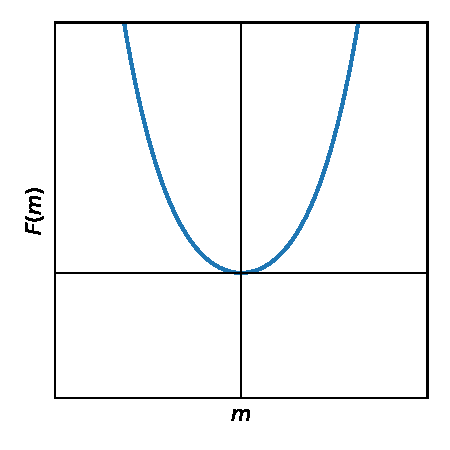
\includegraphics[scale=0.8]{figures/free energy when a(T) is greater than 0.pdf}
			\caption{free energy when $a(T) > 0$.}
		\end{subfigure}
		\begin{subfigure}{0.4\linewidth}
			\centering
			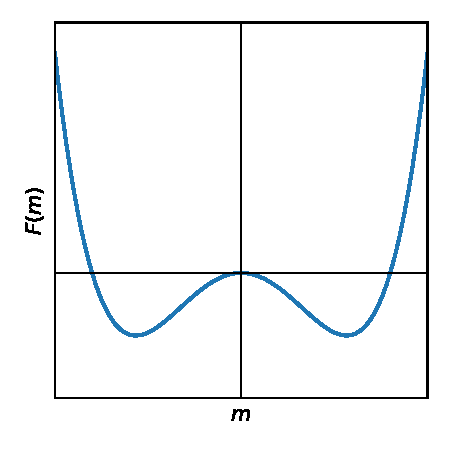
\includegraphics[scale=0.8]{figures/free energy when a(T) is less than 0.pdf}
			\caption{free energy when $a(T) < 0$.}
		\end{subfigure}
		\caption{}
	\end{figure}
	
	\item 将 equilibrium value of $m$ 代入 free energy, 得到
	\begin{equation}
		F(T) = \begin{dcases}
			F_0(T) & T > T_c \\
			F_0(T) - \frac{a^2(T)}{4 b(T)} & T < T_c
		\end{dcases},
	\end{equation}
	可见 $F(T)$ 在 $T = T_c$ 处连续, 且
	\begin{equation}
		\begin{dcases}
			S = - \frac{\partial F}{\partial T} = \begin{dcases}
				F_0'(T) & T < T_c \\
				F_0'(T) - \frac{2 a a' b - a^2 b'}{4 b^2} & T > T_c
			\end{dcases} \\
			\frac{C_V}{T} = \frac{\partial S}{\partial T} = \begin{dcases}
				F_0''(T) & T < T_c \\
				F_0''(T) - \frac{2 a a'' b^2 + 2 a'^2 b^2 - 4 a a' b b' + 2 a^2 b'^2 - a^2 b b''}{4 b^3} & T > T_c
			\end{dcases}
		\end{dcases},
	\end{equation}
	$S$ 连续但 $C_V$ 不连续, 因此是 second order phase transition.
	
	\item 如果假设 $T_c$ 附近
	\begin{equation}
		b = b_0, \quad a = a_0 (T - T_c),
	\end{equation}
	 那么
	 \begin{equation}
	 	m_0 = \pm \sqrt{- \frac{a_0}{2 b_0}} (T - T_c)^{1 / 2},
	 \end{equation}
	 得到 critical exponent $\beta = \frac{1}{2}$.
\end{itemize}

\subsection{spontaneous symmetry breaking}
\begin{itemize}
	\item 在 $T < T_c$ 时, 系统基态处于 $m = \pm m_0$, 此时 $\mathbb{Z}_2$ symmetry is spontaneously broken by the choice of ground state of the theory.
	
	\item 对于 BECs, superfluids, superconductors and Higgs mechanism, $m^2 = |\psi|^2 \geq 0, \psi \in \mathbb{C}$, 系统 (free energy 依然具有 \eqref{11.5.3} 的形式) 具有 $\mathrm{U}(1)$ symmetry.
\end{itemize}

\subsection{first order phase transitions}
\begin{itemize}
	\item 考虑系统的 free energy 含有 odd power terms,
	\begin{equation}
		F(T, m) = F_0(T) + \alpha(T) m + a(T) m^2 + \gamma(T) m^3 + b(T) m^4 + \cdots,
	\end{equation}
	对于 Ising model 有
	\begin{equation}
		F_\text{Ising}(T, m) = - N k_B T \ln 2 + \frac{q N}{2} J m^2 - \frac{N}{2 k_B T} (B + q J m)^2 + \frac{N}{24 (k_B T)^3} (B + q J m)^4 + \cdots,
	\end{equation}
	此时系统不再具有 $\mathbb{Z}_2$ symmetry.
	
	\item 依然假设 $b(T) > 0$ for all $T$.
	
	\item 系统的 ground state 在 $m > 0$ 和 $m < 0$ 之间不连续地变化 (first order phase transition), 这可能由温度改变导致, 也可能是外部参数改变导致. 对于 Ising model, 相变源于 $B$ 的改变.
\end{itemize}

\subsection{Lee--Yang zeros}
\begin{itemize}
	\item 考虑类似 \eqref{11.2.5} 的相互作用, 有限空间中可以容纳的粒子数有限, 最大值为 $N_V \sim V / \sigma^3$.
	
	\item 系统的 grand partition function 为
	\begin{equation}
		Z_\text{GC}(T, V, z) = \sum_{N = 0}^{N_V} z^N Z(T, V, N),
	\end{equation}
	对于 $z$ 是一个 $N_V$ 阶 polynomial, 且系数为正, 因此 $Z_\text{GC}(z)$ 的 zero points 处于实轴负半轴或 complex pairs.
	
	\item 在极限 $V \rightarrow \infty$ 下, $Z_\text{GC}(z)$ 可能有实轴正半轴上的零点.
	
	\item Lee--Yang theorem states that: $Z_\text{GC}(z) \neq 0$ 的区域 (这个区域必须包含实轴正半轴) 里, $\Theta$ 是光滑的; 但如果 $z$ 的实轴正半轴上出现 $Z_\text{GC}(z)$ 零点, 那么 $\Theta$ 一般 not analytic. 其中
	\begin{equation}
		\Theta = \lim_{V \rightarrow \infty} \Big( \frac{1}{V} \ln Z_\text{GC}(T, V, z) \Big).
	\end{equation}
	
	\item $\frac{\partial^n \Theta}{\partial z^n}$ 是最低阶不连续导数, system undergoes $n$\textsuperscript{th} order phase transition.
\end{itemize}

\subsubsection{a made-up example}
\begin{itemize}
	\item 考虑系统的 grand partition function 为
	\begin{equation}
		Z_\text{GC}(V, z) = (1 + z)^{[\alpha V]} (1 + z^{[\alpha V]}),
	\end{equation}
	其中 $[\alpha V]$ 表示 $\alpha V$ 的整数部分, $\alpha$ 是一个与温度有关的参数.
	
	\item $Z_\text{GC}(V, z)$ 的零点为
	\begin{equation}
		z = - 1, \quad \text{and} \quad z = e^{i (2 n + 1) \pi / [\alpha V]}, n = 0, 1, \cdots, [\alpha V] - 1.
	\end{equation}
	
	\item 考虑 $V \rightarrow \infty$, 此时 $z = 1$ 是一个零点, 且
	\begin{align}
		\Theta &= \lim_{V \rightarrow \infty} \Big( \frac{1}{V} ([\alpha V] \ln(1 + z) + \ln(1 + z^{[\alpha V]})) \Big) \notag \\
		&= \begin{dcases}
			\alpha \ln(1 + z) & |z| \leq 1 \\
			\alpha (\ln(1 + z) + \ln z) & |z| > 1
		\end{dcases},
	\end{align}
	可见 $\Theta$ 对所有 $z$ 连续, 但只在 $|z| \neq 1$ 时 analytic.
	
	\item 得到
	\begin{equation}
		\begin{dcases}
			n = z \frac{\partial \Theta}{\partial z} = \begin{dcases}
				\frac{z \alpha}{1 + z} \in [0, {\textstyle \frac{\alpha}{2}}] & z \leq 1 \\
				\frac{\alpha (1 + 2 z)}{1 + z} \in ({\textstyle \frac{3 \alpha}{2}}, 2 \alpha) & z > 1
			\end{dcases} \\
			P = \begin{dcases}
				\alpha k_B T \ln \frac{\alpha}{\alpha - n} & z \leq 1 \\
				\alpha k_B T \ln \frac{2 \alpha n}{(2 \alpha - n)^2} & z > 1
			\end{dcases}
		\end{dcases},
	\end{equation}
	可见系统存在 particle density jump, 类似气液相变.
\end{itemize}

\subsection{Landau--Ginzburg theory}
\begin{itemize}
	\item 考虑 order parameter 具有 fluctuations, 系统依然具有 $\mathbb{Z}_2$ symmetry $m \mapsto - m$, 那么系统的 free energy 为
	\begin{equation}
		F[m(\vec{x})] = \int d^D x \, (a(T) m^2 + b(T) m^4 + c(T) (\nabla m)^2),
	\end{equation}
	其中 $(\nabla m)^2$ 项反应了 nearby spins tend to be aligned.
	
	\item 平衡态下 order parameter 满足 Euler--Lagrange equation,
	\begin{equation} \label{11.5.19}
		c \nabla^2 m = a m + 2 b m^3,
	\end{equation}
	\eqref{11.5.5} 中的结果依然是一种解.
\end{itemize}

\subsubsection{domain walls}
\begin{itemize}
	\item 在 $T < T_c$ 时, $m(\vec{x}) = \pm m_0$ 都是基态, 可能出现系统中一部分处于 $+ m_0$ 其它部分处于 $- m_0$ 的情况 (例如一部分处于气态, 另一部分处于液态).
	
	\item 处于两种基态的部分称为 domain, 交界处称为 domain wall.
	
	\item 考虑 domain wall 附近 $m(\vec{x})$ 的行为, $\hat{n}$ 是 domain wall 的法向矢量, 那么
	\begin{equation}
		c (\hat{n} \cdot \nabla)^2 m = a m + 2 b m^3 \Longrightarrow m = m_0 \tanh \Big( \sqrt{- \frac{a}{2 c}} \hat{n} \cdot \vec{x} \Big).
	\end{equation}
	
	\item domain wall 的厚度为 $\sqrt{- \frac{2 c}{a}}$, 其对 free energy 的贡献为
	\begin{equation}
		\Delta F_\text{domain wall} = L^{D - 1} \sqrt{- \frac{2 c}{a}} \frac{a^2}{3 b},
	\end{equation}
	其中 $L^{D - 1}$ 是 domain wall 的面积.
\end{itemize}

\subsection{correlations}
\begin{itemize}
	\item 计算基态上的一阶扰动, 令 $m(\vec{x}) = m_0 + \delta m(\vec{x})$, 代入 \eqref{11.5.19}, 得到
	\begin{equation}
		c \nabla^2 \delta m + 2 a \delta m = 0,
	\end{equation}
	这个 PDE 的 Green's function 为
	\begin{equation}
		G(\vec{x}) \simeq - \frac{1}{2 (2 \pi)^{(D - 1) / 2} \xi^{(D - 3) / 2}} \frac{e^{- r / \xi}}{r^{(D - 1) / 2}}, \quad r / \xi \gg D, \quad \xi = \sqrt{- \frac{c}{2 a}},
	\end{equation}
	其中 $\xi$ 称为 correlation length, 并注意到 critical point 附近 $a \rightarrow 0, \xi \rightarrow \infty$.
	
	\begin{tcolorbox}[title=calculation:]
		作 Fourier transformation 有
		\begin{equation}
			\Big( - |\vec{k}|^2 + \frac{2 a}{c} \Big) \tilde{G}(\vec{k}) = 1 \Longrightarrow G(\vec{x}) = \int \frac{d^D k}{(2 \pi)^D} \frac{e^{i \vec{k} \cdot \vec{x}}}{- |\vec{k}|^2 + \frac{2 a}{c}},
		\end{equation}
		且
		\begin{align}
			G(\vec{x}) &= \int \frac{d^D k}{(2 \pi)^D} \frac{e^{i \vec{k} \cdot \vec{x}}}{- |\vec{k}|^2 + \frac{2 a}{c}} \notag \\
			&= \frac{1}{(2 \pi)^D} \int d\Omega_{D - 2} \int_0^\pi \sin \theta d\theta \int_0^\infty k^{D - 1} dk \, \frac{e^{i k r \cos \theta}}{- k^2 + \frac{2 a}{c}} \notag \\
			&= \frac{1}{(2 \pi)^D} \frac{2 \pi^{(D - 1) / 2}}{\Gamma(\frac{D - 1}{2})} \frac{2}{r} \int_0^\infty dk \, \frac{k^{D - 2} \sin k r}{- k^2 + \frac{2 a}{c}} = \cdots
		\end{align}
		
		\noindent\rule[0.5ex]{\linewidth}{0.5pt} % horizontal line
		
		另一种方法是引入对 $\alpha$ 的积分 (其中 $\mu = \sqrt{- \frac{2 a}{c}}$),
		\begin{equation}
			\frac{1}{|\vec{k}|^2 + \mu^2} = \int_0^\infty d\alpha \, e^{- \alpha (|\vec{k}|^2 + \mu^2)},
		\end{equation}
		代入, 得到
		\begin{align}
			G(\vec{x}) &= \int \frac{d^D k}{(2 \pi)^D} \frac{e^{i \vec{k} \cdot \vec{x}}}{- |\vec{k}|^2 + \frac{2 a}{c}} = - \int_0^\infty d\alpha \, e^{- \alpha \mu^2} \int \frac{d^D k}{(2 \pi)^D} e^{- \alpha |\vec{k}|^2 + i \vec{k} \cdot \vec{x}} \notag \\
			&= - \int_0^\infty d\alpha \, \frac{e^{- \alpha \mu^2 - \frac{r^2}{4 \alpha}}}{(4 \pi \alpha)^{D / 2}} = - \frac{1}{(2 \pi)^{D / 2}} \Big( \frac{\mu}{r} \Big)^{\frac{D - 2}{2}} K_{\frac{D - 2}{2}}(\mu r),
		\end{align}
		其中 $K$ 是 \href{https://en.wikipedia.org/wiki/Bessel_function#Modified_Bessel_functions:_I%CE%B1,_K%CE%B1}{modified Bessel functions of the second kind}. 在 $\mu r \gg D$ 的情况下, 将积分写作
		\begin{equation}
			G(\vec{x}) = - \frac{1}{(4 \pi)^{D / 2}} \int_0^\infty d\alpha \, e^{f(\alpha)}, \quad f(\alpha) = - \alpha \mu^2 - \frac{r^2}{4 \alpha} - \frac{D}{2} \ln \alpha,
		\end{equation} 
		$f(\alpha)$ 的最小值位于 $\alpha_0 = \frac{- D + \sqrt{D^2 + 4 \mu^2 r^2}}{4 \mu^2} \simeq \frac{r}{2 \mu}$, 此时
		\begin{equation}
			f(\alpha_0) \simeq - \mu r - \frac{D}{2} \ln \frac{r}{2 \mu}, \quad f''(\alpha_0) \simeq - \frac{4 \mu^3}{r} + O(r^{- 2}),
		\end{equation}
		因此
		\begin{equation}
			G(\vec{x}) \simeq - \frac{1}{(4 \pi)^{D / 2}} \Big( \frac{2 \mu}{r} \Big)^{\frac{D}{2}} e^{- \mu r} \sqrt{\frac{\pi r}{2 \mu^3}} = - \frac{\mu^{(D - 3) / 2}}{2 (2 \pi)^{(D - 1) / 2}} \frac{e^{- \mu r}}{r^{(D - 1) / 2}}.
		\end{equation}
	\end{tcolorbox}
\end{itemize}

\subsection{fluctuations}
\begin{itemize}
	\item Landau theory 中的 free energy 可以由下式定义,
	\begin{equation}
		e^{- \beta F[m(\vec{x})]} = \sum_{\{s_i\} | m(\vec{x})} e^{- \beta E\{s_i\}},
	\end{equation}
	那么 partition function 可以用 functional integral 表示为
	\begin{equation}
		Z_\text{C} = e^{- \beta F} = \int Dm \, e^{- \beta F[m(\vec{x})]}.
	\end{equation}
\end{itemize}
